\documentclass[10pt,dvipsnames,enabledeprecatedfontcommands]{scrartcl}
\usepackage{lmodern}
\usepackage{amssymb,amsmath}
\usepackage{ifxetex,ifluatex}
\usepackage{fixltx2e} % provides \textsubscript
\ifnum 0\ifxetex 1\fi\ifluatex 1\fi=0 % if pdftex
  \usepackage[T1]{fontenc}
  \usepackage[utf8]{inputenc}
\else % if luatex or xelatex
  \ifxetex
    \usepackage{mathspec}
  \else
    \usepackage{fontspec}
  \fi
  \defaultfontfeatures{Ligatures=TeX,Scale=MatchLowercase}
\fi
% use upquote if available, for straight quotes in verbatim environments
\IfFileExists{upquote.sty}{\usepackage{upquote}}{}
% use microtype if available
\IfFileExists{microtype.sty}{%
\usepackage[]{microtype}
\UseMicrotypeSet[protrusion]{basicmath} % disable protrusion for tt fonts
}{}
\PassOptionsToPackage{hyphens}{url} % url is loaded by hyperref
\usepackage[unicode=true]{hyperref}
\PassOptionsToPackage{usenames,dvipsnames}{color} % color is loaded by hyperref
\hypersetup{
            pdftitle={Likelihood ratio and evidence strength},
            pdfauthor={Marcello Di Bello and Rafal Urbaniak},
            colorlinks=true,
            linkcolor=Maroon,
            citecolor=Blue,
            urlcolor=blue,
            breaklinks=true}
\urlstyle{same}  % don't use monospace font for urls
\usepackage{graphicx,grffile}
\makeatletter
\def\maxwidth{\ifdim\Gin@nat@width>\linewidth\linewidth\else\Gin@nat@width\fi}
\def\maxheight{\ifdim\Gin@nat@height>\textheight\textheight\else\Gin@nat@height\fi}
\makeatother
% Scale images if necessary, so that they will not overflow the page
% margins by default, and it is still possible to overwrite the defaults
% using explicit options in \includegraphics[width, height, ...]{}
\setkeys{Gin}{width=\maxwidth,height=\maxheight,keepaspectratio}
\IfFileExists{parskip.sty}{%
\usepackage{parskip}
}{% else
\setlength{\parindent}{0pt}
\setlength{\parskip}{6pt plus 2pt minus 1pt}
}
\setlength{\emergencystretch}{3em}  % prevent overfull lines
\providecommand{\tightlist}{%
  \setlength{\itemsep}{0pt}\setlength{\parskip}{0pt}}
\setcounter{secnumdepth}{5}
% Redefines (sub)paragraphs to behave more like sections
\ifx\paragraph\undefined\else
\let\oldparagraph\paragraph
\renewcommand{\paragraph}[1]{\oldparagraph{#1}\mbox{}}
\fi
\ifx\subparagraph\undefined\else
\let\oldsubparagraph\subparagraph
\renewcommand{\subparagraph}[1]{\oldsubparagraph{#1}\mbox{}}
\fi

% set default figure placement to htbp
\makeatletter
\def\fps@figure{htbp}
\makeatother

%\documentclass{article}

% %packages
 \usepackage{booktabs}

\usepackage{multirow}
\usepackage{colortbl}
\usepackage{graphicx}
\usepackage{longtable}
\usepackage{ragged2e}
\usepackage{etex}
%\usepackage{yfonts}
\usepackage{marvosym}
\usepackage[notextcomp]{kpfonts}
\usepackage{nicefrac}
\newcommand*{\QED}{\hfill \footnotesize {\sc Q.e.d.}}
\usepackage{floatrow}

\usepackage[textsize=footnotesize]{todonotes}
\newcommand{\ali}[1]{\todo[color=gray!40]{\textbf{Alicja:} #1}}

%\linespread{1.5}
\newcommand{\indep}{\!\perp \!\!\! \perp\!}


\setlength{\parindent}{10pt}
\setlength{\parskip}{1pt}


%language
\usepackage{times}
\usepackage{t1enc}
%\usepackage[utf8x]{inputenc}
%\usepackage[polish]{babel}
%\usepackage{polski}




%AMS
\usepackage{amsfonts}
\usepackage{amssymb}
\usepackage{amsthm}
\usepackage{amsmath}
\usepackage{mathtools}

\usepackage{geometry}
 \geometry{a4paper,left=35mm,top=20mm,}


%environments
\newtheorem{fact}{Fact}



%abbreviations
\newcommand{\ra}{\rangle}
\newcommand{\la}{\langle}
\newcommand{\n}{\neg}
\newcommand{\et}{\wedge}
\newcommand{\jt}{\rightarrow}
\newcommand{\ko}[1]{\forall  #1\,}
\newcommand{\ro}{\leftrightarrow}
\newcommand{\exi}[1]{\exists\, {_{#1}}}
\newcommand{\pr}[1]{\mathsf{P}(#1)}
\newcommand{\cost}{\mathsf{cost}}
\newcommand{\benefit}{\mathsf{benefit}}
\newcommand{\ut}{\mathsf{ut}}

\newcommand{\odds}{\mathsf{Odds}}
\newcommand{\ind}{\mathsf{Ind}}
\newcommand{\nf}[2]{\nicefrac{#1\,}{#2}}
\newcommand{\R}[1]{\texttt{#1}}
\newcommand{\prr}[1]{\mbox{$\mathtt{P}_{prior}(#1)$}}
\newcommand{\prp}[1]{\mbox{$\mathtt{P}_{posterior}(#1)$}}



\newtheorem{q}{\color{blue}Question}
\newtheorem{lemma}{Lemma}
\newtheorem{theorem}{Theorem}



%technical intermezzo
%---------------------

\newcommand{\intermezzoa}{
	\begin{minipage}[c]{13cm}
	\begin{center}\rule{10cm}{0.4pt}



	\tiny{\sc Optional Content Starts}
	
	\vspace{-1mm}
	
	\rule{10cm}{0.4pt}\end{center}
	\end{minipage}\nopagebreak 
	}


\newcommand{\intermezzob}{\nopagebreak 
	\begin{minipage}[c]{13cm}
	\begin{center}\rule{10cm}{0.4pt}

	\tiny{\sc Optional Content Ends}
	
	\vspace{-1mm}
	
	\rule{10cm}{0.4pt}\end{center}
	\end{minipage}
	}
%--------------------






















\newtheorem*{reply*}{Reply}
\usepackage{enumitem}
\newcommand{\question}[1]{\begin{enumerate}[resume,leftmargin=0cm,labelsep=0cm,align=left]
\item #1
\end{enumerate}}

\usepackage{float}

% \setbeamertemplate{blocks}[rounded][shadow=true]
% \setbeamertemplate{itemize items}[ball]
% \AtBeginPart{}
% \AtBeginSection{}
% \AtBeginSubsection{}
% \AtBeginSubsubsection{}
% \setlength{\emergencystretch}{0em}
% \setlength{\parskip}{0pt}






\usepackage[authoryear]{natbib}

%\bibliographystyle{apalike}



\usepackage{tikz}
\usetikzlibrary{positioning,shapes,arrows}

\title{Likelihood ratio and evidence strength}
\author{Marcello Di Bello and Rafal Urbaniak}
\date{}

\begin{document}
\maketitle

{
\hypersetup{linkcolor=black}
\setcounter{tocdepth}{2}
\tableofcontents
}
\tableofcontents

\todo{Read and discuss the decision Marcello sent}
\todo{paragraph on implementation of false positive ratios, LR guides us in further research}
\todo{Allen objection to infinite complexity, plausibility and probability?,  The nature of juridical proof: Probability as a tool in plausible reasoning, s intuitive, reduction of complexities in choosing hypotheses in LR}
\todo{Move cold hit into the appendix}
\todo{Sprinkle the confirmation measures over section two, move to appendix}
\todo{write the conclusions section}

\section{Introduction}\label{introduction}

Our goal in this chapter is to take a closer look at an important tool
of evidence evaluation proposed by legal probabilists: the likelihood
ratio. In Section \ref{sec:lr} we explain what this measure of
evidential strength is, how it compares to another one, sometimes called
the Bayes factor, and why it is preferable to it. In Section
\ref{sec:fp} we give an example of its utility. We explain the reasons
to take the risk of false positives in DNA identification seriously and
use likelihood ratio to illustrate the impact of such a risk on the
value of DNA evidence. Another example, developed in Section
\ref{sec:eyewitness}, is meant to remove the impression that likelihood
ratios are useful only for clearly quantitative evidence such as DNA
evidence. We talk about the insights that probabilistic thinking can
bring into eyewitness evidence evaluation and incorporation.

Likelihood ratio, while useful, is sometimes hard to interpret in
practice, as it depends on the choice of the hypotheses involved. We
discuss this problem in Section \ref{sec:hchoice}. One reason why many
hypotheses can be considered in such contexts is that they admit
different levels: we discuss this phenomenon in Section
\ref{sec:lhTwoSTain}, illustrating it with the example of the so-called
two-stain problem. The general lesson from these sections is that
likelihood ratio, while a very useful measure of evidential value, when
presented alone without proper attention paid to hypothesis formulation
and the impact of the choice of the hypotheses on the likelihood ratio
itself, might be misleading.

Next, in Section \ref{sec:relevance} we discuss another problem put
forward against the utility of likelihood ratios: the problem of
relevance. On this objection, likelihood ratio sometimes fails to
identify all the relevant items of evidence. We explain what the
objection is, and why it is misled. However, the discussion leads us to
another reason why likelihood ratio when presented alone might be
unhelpful. Indeed, it might be the case that a piece of evidence is
irrelevant with respect to a certain choice of hypotheses, but relevant
to another, and all of these hypotheses might play an important role in
the fact-finding process. As relevance is to be established in
connection with various elements of a complex case, instead of a single
likelihood ratio, one should consider various likelihood ratios arising
for various selections of hypotheses at play, and so a readable
representation of such complexities involved in a given case would be
useful for putting various likelihood ratios to a proper use.

To illustrate the utility of thinking in terms of likelihood ratios in
theorizing about the value of evidence, we go over a debate about the
value of cold-hit DNA matches in which various agencies studying or
performing DNA evaluation have still failed to reach agreement (Section
\ref{sec:coldHitConfusion}), and argue that a proper use of likelihood
ratios leads to a fairly clear resolution (Section \ref{sec:cold-hit}).

We end this chapter with two digressions. Another is meant for a more
philosophically minded reader, who might recall that there are quite a
few probabilistic confirmation measures in the vincinity and might
wonder why almost none of them were discussed in the chapter. In Section
\ref{sec:confirmation} we explain why we think these other measures are
not fit for the particular purpose at hand: evidence evaluation in
legal-fact finding.

\section{\texorpdfstring{Likelihood ratio as a measure of evidence
strength
\label{sec:lr}}{Likelihood ratio as a measure of evidence strength }}\label{likelihood-ratio-as-a-measure-of-evidence-strength}

The fallacies we considered earlier in the book \todo{add crossref}---
such as the base rate fallacy, the prosecutor's fallacy, and the defense
attorney's fallacy---show how the posterior probability can be
misjudged, upwards or downwards, even if the subject gets the
likelihoods right. These examples illustrate that the assessment of the
posterior probability of a hypothesis given the evidence depends also on
the prior probability of the hypothesis. The correctness of such an
assessment therefore requires that the priors are chosen sensibly (or
that a range of sensible priors is considered) and appropriately put
together with the likelihoods involved. Quite crucially, the posterior
probability given a piece of evidence should not be confused with the
probative value of a given piece of evidence itself with respect to the
hypothesis in question.

Consider the following examples. Suppose the prior probability of a
given hypothesis \(H\) is low, say \(\pr{H}=.001\), but taking evidence
\(E\) into account brings this probability up to \(.35\), that is,
\(\pr{H \vert E}=.35\). This is a dramatic upward shift. Even though the
posterior probability of \(H\) given \(E\) is not very high, \(E\)
strongly favors \(H\). Conversely, suppose the prior probability of
\(H\) is extremely high, say \(\pr{H}=.999\), but taking evidence \(E\)
into account brings this probability down to \(.75\), that is,
\(\pr{H \vert E}=.75\). This is a dramatic downward shift. Even though
the posterior probability of \(H\) given \(E\) is still quite high,
\(E\) speaks against \(H\). Now, let's turn to the blood stain example
from \ref{sec:fallacies}.\todo{Fix crossref.} The posterior probability
given the match turned out to be an unimpressive \(.17\) (assuming a
prior probability of \(.1\)). This does not mean that the incriminating
evidence was weak. While the match was not not strong enough to make it
very likely that the defendant was the source of the traces, the
posterior probability is seventeen times larger than the prior.
Similarly, in the Collins case, the posterior probability jumped from
the \(\nicefrac{1}{6 \times 10^6}\) prior to \(.7\) after taking the
match into account. Still not enough for a conviction, but a remarkable
increase nonetheless. These examples illustrate how measuring the
strength of evidence in terms of the posterior it leads to seems
inappropriate.

So how do we capture the strength of an item of evidence that reflects
the impact the evidence on the posterior probability? One measure of the
strength of evidence is the likelihood of the evidence compared to the
prior of the evidence (this measure is sometimes called the
\emph{Bayes factor}:

\begin{align}\label{eq:BF}
\tag{BF}
\mathsf{BF}(E,H) & = \frac{\pr{E \vert H}}{\pr{E}}.
\end{align}

\noindent The Bayes factor is one probabilistic measure of the extent to
which the evidence, regardless of the absolute posterior probability,
supports or does not support the hypothesis. It seem to be an
intuitively plausible measure of evidential strength. Note that by
Bayes' theorem

\vspace{-3mm}

\begin{align*}
\pr{H \vert E} & = \mathsf{BF}(H, E) \times \pr{H}
\end{align*}

\noindent and so the Bayes factor is greater than one if and only if the
posterior probability \(\pr{H \vert E}\) is higher than the prior
probability \(\pr{H}\), \(\pr{H}<\pr{H\vert E}\). So \(E\)
\textit{positively} supports \(H\) whenever the Bayes factor is greater
than one. The greater the Bayes factor (for values above one), the
greater the upward shift from prior to posterior probability, the more
strongly \(E\) positively supports \(H\). In line with the motivating
examples, the posterior probability of \(H\) given \(E\) could still be
low even if the Bayes factor is significantly above one. Conversely,
again by Bayes' theorem, the probability of \(H\) given \(E\) is lower
than the probability of \(H\), \(\pr{H}>\pr{H\vert E}\) just in case the
Bayes factor is less than one. So \(E\) \textit{negatively} supports
\(H\) whenever the Bayes factor is less than one. In general, the
smaller the Bayes factor (for values below one), the greater the
downward shift from prior to posterior probability, the more strongly
\(E\) negatively supports \(H\). If \(\pr{H}=\pr{H\vert E}\), the
evidence has no impact on the probability of \(H\).

One reason to think the Bayes Factor is a useful measure of evidential
strength is that it appropriately deviates from 1, its point of
neutrality. But let us pause a moment to think about the denominator in
\eqref{eq:BF}. It can be calculated following the law of total
probability:

\vspace{-3mm}

\begin{align} \label{eq:lotpSimple}
\pr{E}= \pr{E \vert H} \pr{H}+\pr{E \vert \neg H} \pr{\neg H}.
\end{align}

\noindent The catch-all alternative hypothesis \(\neg H\) can be
replaced by a more fine-grained set of alternatives, say
\(H_1, H_2, \dots H_k\), provided \(H\) and these alternatives are
exclusive and cover the entire space of possibilities (that is, they
form a partition). The law of total probability would then read:

\begin{align} \label{eq:lotpLong}
\pr{E} & = \pr{E\vert H}\pr{H} +\sum_{i=1}^k \pr{E\vert H_i}\pr{H_i}. 
\end{align}

\noindent For simplicity, let's stick to \eqref{eq:lotpSimple} for now,
and use it to rewrite \eqref{eq:BF}:

\begin{align}\label{eq:BFlotp}
\mathsf{BF}(E,H) & = \frac{\pr{E \vert H}}{\pr{E \vert H} \pr{H}+\pr{E \vert \neg H} \pr{\neg H}}.
\end{align}

\noindent What should be clear from this formulation is that the Bayes
factor depends on the prior probabilities. Indeed, suppose
\(\pr{E \vert H} = 1\) and \(\pr{E \vert \neg H} = .1\). If
\(\pr{H}=.1\), \(\pr{E}\), the denominator, is \(.19\) and so the Bayes
Factor is approximately \(5.26\). If, however, \(\pr{H} =.2\), the
denominator is \(.28\) and the Bayes Factor is approximately \(3.57\).
In fact, a more general look (Figure \ref{fig:BayesFactorPrior}) shows
the prior probability can have larger impact on the Bayes factor than
the likelihood \(\pr{E \vert \n H}\).

This seems to be a reason against using the Bayes factor as a measure of
evidential strength in the context of legal fact-finding. After all, in
such contexts, we would like the expert's assessment not to depend on
the expert's prior convictions about the hypothesis, and for all the
agents involved in legal fact-finding to understand the expert's
statement in the same way, even if they assign different priors to the
hypothesis.
\todo{Think about this again later. Plausible, but I think this needs some more careful discussion. Diagnostic properties of medical tests might change depeding on base rate?}

\footnotesize

\normalsize 

\begin{figure}


\begin{center}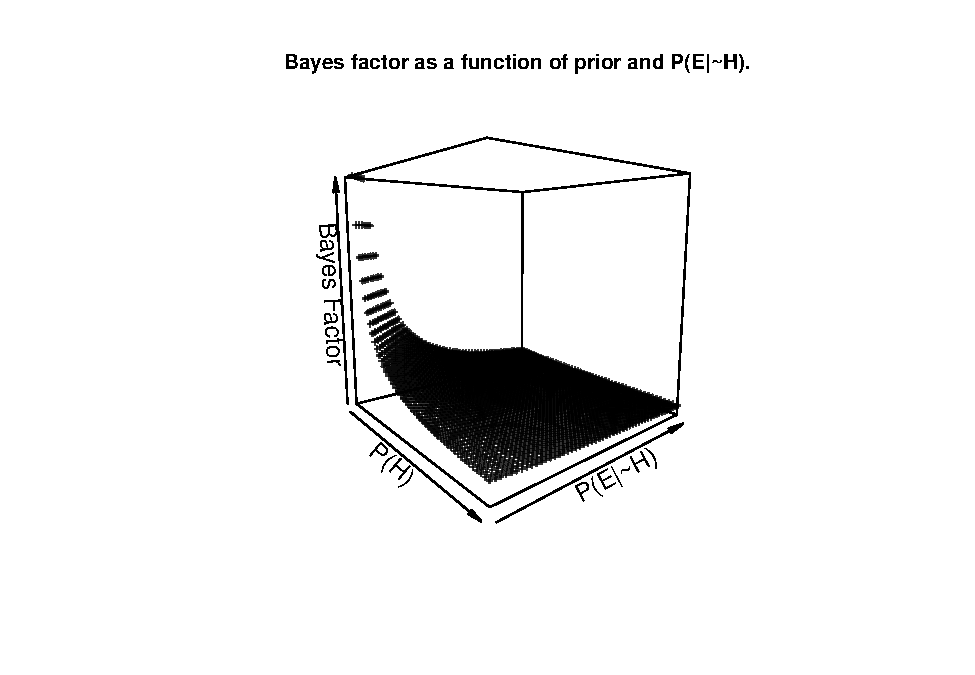
\includegraphics[width=1\linewidth]{lr-chapter3_files/figure-latex/fig-BayesFactorPrior-1} \end{center}
\caption{Impact of the prior and likelihood of E given ~H for probabilities in (0, 0.05) and Bayes Factor restricted to (0, 250) for visibility.}
\label{fig:BayesFactorPrior}
\end{figure}

\noindent A related reason to worry about the denominator of
\eqref{eq:BFlotp} is that assessing the strength of evidence using the
Bayes factor seems to impose too great a cognitive burden on an agent,
since it would require estimating \(\pr{E}\). This rarely can be done
directly, and estimation using the denominator of \eqref{eq:BFlotp} or
\eqref{eq:lotpLong} (in a more complex case) not only requires that the
agent sifts through the entire space of possibilities, but also that the
agent uses as weights a sensible selection of priors for the hypotheses
involved.

Here is another reason to hestitate about measuring evidential support
with \textsf{BF}, stemming from (Gillies, 1986).\footnote{See also
  (Fitelson, 1999) for a discussion.} Consider the hypothesis \(H =:\)
``the suspect is guilty'' and suppose it is already known that \(E =:\)
``the suspect killed the victim'' (say here guilt requires both
\emph{actus reus}, the killing, and \emph{mens rea}, the intention).
Clearly, \(H\) entails \(E\), and \(E\) provides positive support for
\(H\). Now consider a composite hypothesis \(H'=:\) ``the suspect is
guilty and we live in a simulation built by aliens.'' We hope the reader
shares the intuition that the support \(E\) provides for \(H'\) is
somewhat weaker than it does for \(H\) (yes, the example of \(H'\) is
really far-fetched, but this is the point: addition of far-fetched
hypotheses should decrease the support). This feature, however, cannot
be captured by \textsf{BF}. In general, suppose \(H\models E\) (and so,
also, \(H \et X \models E\)). Then both \(\pr{E\vert H}\) and
\(\pr{E \vert H \et X}\) equal 1. But this means that
\(\mathsf{BF}(H,E) = \mathsf{BF}(H \et X, E) = \nicefrac{1}{\pr{E}}\),
and so the Bayes factors for the two support relations are equal.

We will paint a more complex picture of various confirmation measures
and the conditions they satisfy in Section \ref{sec:confirmation}. For
now, we will focus on motivating and investigationg the one that has
been actually used by legal probabilists: the likelihood ratio.

Suppose we are after a measure that does not depend on priors, puts no
such cognitive requirements on an agent, and is sensitive to the
addition of irrelevant conjuncts. Clearly, we should not simply use
\(\pr{E\vert H}\). For one thing, in many interesting cases this
conditional probability will be very close to one and will not allow us
to distinguish between the strenghts of pieces of evidence that we
should distinguish. For instance, what is the probability that the blood
types match if the accussed is the source? Well, one, pretty much. What
is the probability that the DNA profiles match if the accussed is the
source? Again, one, pretty much. But obviously a DNA profile match is
not on par with a blood type match insofar as strength of evidence is
involved.

Even if this conditional probability is not close to one, there are
reasons not to use it as a measure of evidential strength. Consider an
example by Triggs \& Buckleton (2004). In a child abuse case, the
prosecutor offers \label{text:rock} evidence that a couple's child rocks
and that only 3\% of non-abused children rock,
\(\pr{\textsf{child rocks} \vert \textsf{no abuse}}=.3\). If it is
unlikely that a non-abused child would rock, the fact that this child
rocks might seem strong evidence of abuse. But this reading of the 3\%
figure is mistaken. It could well be that 3\% of abused children rock,
\(\pr{\textsf{child rocks} \vert \textsf{abuse}}=.3\). Note that the two
probabilities need not add up to 1. Similarly, learning only that
\(\pr{\textsf{child rocks} \vert \textsf{abuse}}=.3\) does not provide
full information needed for evidence evaluation, and one also needs
information about
\(\pr{\textsf{child rocks} \vert \textsf{no abuse}}=.3\). In our
particular case, given that rocking is equally unlikely under either
hypothesis, rocking cannot count as evidence of abuse, and any of the
low conditional probabilities involved alone does not allow us to notice
this. Thus, in order to avoid exaggerations of the evidence both
conditional probabilities need to be involved in the evidence strength
evaluation (ENFSI, 2015; Royall, 1997; Triggs \& Buckleton, 2004).

One issue that these considerations illustrate is that what matters is
also the probability of the evidence if the hypothesis is false. If the
accussed is not the source, the probability of a blood match if the
accussed is not the source, while small, is much higher than the
probability of a DNA profile match, and this seems to explain why the
latter piece of evidence is stronger. So, both the probability of the
evidence given the hypothesis, and the probability of evidence given an
alternative hypothesis should be somehow factored into a useful measure
of evidential strength.

One straightforward way to implement this is to use the
\textbf{likelihood ratio}, a comparative measure of whether evidence
\(E\) supports a hypothesis \(H\) more than a competing hypothesis
\(H'\), in symbols:

\begin{align}
\label{eq:LR}
\tag{LR}
\mathsf{LR}(E,H,H') & = \frac{\pr{E \vert H}}{\pr{E \vert H'}}.
\end{align}

\noindent If the evidence supports \(H\) more than \(H'\), the ratio
would be above one, and if the evidence supports \(H'\) more than \(H\),
the ratio would be below one. So, as with the Bayes factor , support
levels correspond to deviations from one. The greater the likelihood
ratio (for values above one), the stronger the evidence in favor of
\(H\) as contrasted with \(H'\). The smaller the likelihood ratio (for
values below one), the stronger the evidence in favor of the competing
hypothesis \(H'\) as contrasted with \(H\).

One reason to prefer \textsf{LR} to \textsf{BF} is that \textsf{LR} is
not susceptible to the addition of irrelevant hypotheses. Even if
\(\pr{E\vert H} = \pr{E\vert H \et X} = 1\), we have that
\(\mathsf{LR}(E,H) = \nicefrac{1}{\pr{E \vert \n H}}\), while
\(\mathsf{LR}(E, H \et X) = \nicefrac{1}{\pr{E \vert \n H \vee \n X}}\).
Crucially, the denominators might differ and so might the resulting
likelihoods.

The likelihood ratio does not depend on the priors, and is a simpler and
more workable measure than the Bayes factor, since it does not require
one to think about the probability of the evidence in general, namely
\(\pr{E}\). Think of blood match evidence. To calculate the Bayes
factor, we need two things: \(\pr{E\vert H}\), which here---say---is
close to one, and \(\pr{E}\), which is the probability of a blood match
\emph{not} conditional on whether the suspect is the source. Yet, direct
and reliable estimation of this probability seems to be quite hard. Of
course, one could try to use the law of total probability, as in
\eqref{eq:lotpSimple}, but then they would need to use
\(\pr{E\vert \n H}\) which, with \(\pr{E\vert H}\), would already
suffice for the calculation of \textsf{LR}, and additional information
about other probabilities used in the right-hand side. In this sense, it
seems that the calculation of \textsf{BF} is more committing and
requires more information than the calculation of \textsf{LR}.

This apparent simplicity of \textsf{LR}, however, can often give rise to
errors in the assessment of the evidence, especially if the two
hypotheses are not chosen carefully. As it will transpire, the choice of
the hypotheses that are conditioned upon is crucial. In the most
straightforward case, \(H'\) is simply the negation of \(H\). In many
practical contexts such a simplistic set-up, however, is not viable. We
will discuss these issues in detail in this chapter later on.

Moreover, \textsf{LR} allows for a clearer separation of the impact of
the priors from the impact of the evidence on the posterior probability.
The relationship between likelihood ratio
\(\nicefrac{\pr{E \vert H}}{\pr{E \vert H'}}\) and posterior odds
\(\nicefrac{\pr{H \vert E}}{\pr{H' \vert E}}\) is apparent in the odds
version of Bayes' theorem:

\begin{align}\label{eq:BTodds}
\frac{\pr{H \vert E}}{\pr{H' \vert E}}= \frac{\pr{E \vert H}}{\pr{E \vert H'}}\times \frac{\pr{H}}{\pr{H'}}.
\end{align}

\noindent If the likelihood ratio is greater (lower) than one, the
posterior odds will be greater (lower) than the prior odds of \(H\). The
likelihood ratio, then, is a measure of the upward or downward impact of
the evidence on the prior odds of two hypotheses \(H\) and \(H'\).

Moreover, the division of labour in legal fact-finding also seems to
recommend \textsf{LR} over \textsf{BF}. A prominent forensic scientist
recommends that `in criminal adjudication, the values of the prior odds
and the posterior odds are matters for the judge and jury, in accordance
with the normal division of labour in forensic fact-finding.' (Aitken \&
Taroni, 2008, p. 194) and that the experts should `not trespass on the
province of the jury by commenting directly on the accused's guilt or
innocence, \dots and should generally confine their testimony to
presenting the likelihood of their evidence under competing
propositions' (Aitken, Roberts, \& Jackson, 2010, p. 42). If however,
the expert were to report \textsf{BF}, this would mean they are
competent to estimate \(\pr{E}\) directly, which is unlikely, or that
they implicitly estimate it relying on their estimation of \(\pr{H}\) in
the background (if they use the law of total probability). In contrast,
\textsf{LR} is one way to describe the value of evidence while abiding
by these constraints, and it in fact is used in practice. Experts
sometimes do testify by offering the likelihood ratio as a measure of
the strength of the evidence. An expert, for instance, may testify that
the blood-staining on the jacket of the defendant is ten times more
likely to be seen if the wearer of the jacket hit the victim
(prosecutor's hypothesis) rather than if he did not (defense's
hypothesis) (Aitken et al., 2010, p. 38).

The idea that both conditional probabilities involved in likelihood
ratio should be used in evidence strength evaluation applies generally
to all forms of evidence, inclusive of DNA evidence, although it might
not always make a practical difference. For suppose an expert testifies
that the crime traces genetically match the defendant and that the
\textbf{random match probability} is extremely low, say 1 in 100
million. Is the match strong evidence that the defendant is the source
of the traces? The random match probability---often interpreted as the
probability that someone who is not the source would coincidentally
match, \(\pr{\textsf{match} \vert \neg \textsf{source}}\)---is a common
measure of the strength of a DNA match. The lower this probability, the
more strongly incriminating the match. This is sensible because a low
random match probability suggests it is unlikely two people could share
the same DNA profile. This is, however, also in agreement with the use
of likelihood ratio in evidence evaluation, because
\(\pr{\textsf{match} \vert \textsf{source}}\) is practically equal to
one, so neglecting in in evidence strength reporting does not make any
real difference. That \(\pr{\textsf{match} \vert \neg \textsf{source}}\)
is low is in such contexts enough to ensure that the likelihood ratio is
significantly above one. For practical purposes, then, a suitably low
random match probability does capture the idea that the evidence is
strongly incriminating evidence. The conceptual point still stands,
though. If \(\pr{\textsf{match} \vert \textsf{source}}\) was
significantly different from one, reporting only
\(\pr{\textsf{match} \vert \neg \textsf{source}}\) would be misleading.

Our goal in this chapter is to reach a balanced view of the utility of
\textsf{LR}. On one hand, we want to motivate its use and appreciate its
utility. On the other, we want to point out reasons why \textsf{LR}
might be misleading or unhelpful. In the next subsection, we will focus
on a part of the positive task. A good example of the positive role of
textsf\{LR\} in theorizing about fact-finding is its the use in studying
the impact of false positive risk. We will take a look at this example
now, in Section \ref{sec:fp}. Later on (Section
\ref{sec:coldHitConfusion}), we will take a more detailed look at
another positive example, the use of \textsf{LR} in studying the value
of the so-called cold-hit matches.\footnote{In principle, it would be
  possible to go over analogous considerations in terms of \textsf{BF},
  however, as we already argued, there are reasons to prefer the use
  \textsf{LR}, and calculations in terms of \textsf{LR} are simpler and
  assume that less information is available to the agent than those in
  terms of \text{BF}.}

\vspace{3mm}
\textbf{Marcello: These first two sections are fine, more or less. They make a clear overall case in favor of LR. Perhpas the second section should come first and then the intro after. The second section motivates looking into LR more closely, which is what we do in the rest of the chapter. The bit about irrelevant conjuction and LR is not clearly explained and needs further elaboration. }

\section{\texorpdfstring{The risk of false positive and its impact
\label{sec:fp}}{The risk of false positive and its impact }}\label{the-risk-of-false-positive-and-its-impact}

One context in which probabilities are extensively used is the use of
DNA evidence. In testifying about the DNA match at trial, experts often
assess the probability that a random person, unrelated to the crime,
would coincidentally match the crime stain profile (random match
probability). RMP is often an impressively low number, say 1 in 100
million or lower. Usually, such a match is taken to constitute strong
evidence against the defendant. We will have more to say about the
interpretation of DNA evidence later on. \todo{add crossref} For now, we
will illustrate the utility of likelihood ratios by using to explain how
this apparent strength of DNA evidence can be mitigated by the
probability of a false positive.

First, observe that while DNA evidence seems as scientific as it gets,
the risk of a false positive is not negligible (Shaer, 2016). For
instance, Houston Police Department Crime Laboratory, a large public
forensic center in Texas, handles around 500 cases a year. In 2016, KHOU
11, a local television station, sent dozens of profiles processed by the
lab to independent experts. The results were not optimistic: police
technicians quite systematically misinterpreted samples.

One notorious case involving a false positive is that of Josiah Sutton
(then 16) and Gregory Adams (then 19), who were arrested for a rape of a
41-year-old woman. The victim was abducted in a parking lot and
assaulted in a driving car (Ford Expedition). A few days after the
incident, the victim spotted Sutton and Adams walking down a street,
flagged down a patrol car, and accussed them of the assault. Both Sutton
and Adams had alibis, neither of them matched the victim's original
description of the perpetrators. Sutton and Adams agreed to a DNA test
to clear their names. A Houston lab analyst Christy Kim compared their
results with DNA obtained from a vaginal swab, which contained a mixture
of genetic material from at least three contributors, including the
victim herself. The lab report did not report a match for Adams, but
concluded that Sutton's DNA was consistent with the mixture DNA. In
result, in 1999, Sutton was sentenced to 25 years in prison. Later on, a
re-examination by prof. William Thompson, indicated that the three DNA
profiles typed by Kim (two from blood, one from saliva) varied, despite
reportedly coming from a single source. Moreover, Kim failed to report
that the DNA from the semen found on the car seat did not match that of
Sutton. In effect, the DNA evidence was reprocessed, no DNA match was
found, and in 2003 Sutton was released from prison.\footnote{Christy Kim
  later on sued her employer for her firing that resulted and won, her
  mistakes being atttributed to systemic failures and inadequate
  supervision.}

This is only one example of quite a few cases of DNA matching going
awry, \todo{cite Inside the Cell, elaborate} and the existing anecdotal
evidence suggests there are quite a few potential sources of error (see
Thompson, 2013 for a more exhaustive treatment and multiple examples):

\begin{itemize}
\item
  \textbf{Cross-contamination of samples.} For instance, in Dwayne
  Johnson (2003) samples were accidentally swapped. In Lukis Anderson
  (2012) the material has been carried over by the responding
  paramedics. In one case, German police invested a considerable amount
  of time and effort searching for the so-called Phantom of Heilbronn,
  whose DNA profile was found on evidence from a large variety of
  crimes. A bountly of 300k EUR was placed on hear head. It turned out
  she was an innocent employee involved in the production of cotton
  swabs used accross the country.
\item
  \textbf{Mislabeling of samples.} For instance, in 2011 the Las Vegas
  Metropolitan Police Department acknowledge that samples of two men
  suspected of a 2001 robbery were switched, leading to the exclusion of
  the perpetrator and four years of incarceration of the other suspect.
  The mistake came to light only because the perpetrator was later on
  arrested for an unrelated crime. In a high-profile case of a serial
  rapist, the notorious Night Stalker who committed more than 140 sexual
  assualts in London, the actual perpertrator came to the attention of
  the police quite soon, but a DNA test excluded him (falsely so,
  because the samples had been mistakenly switched), and so his spree
  continued for months.
\item
  \textbf{Misinterpretation of test results.} While single-source sample
  comparison is not too prone to this sort of error, the interpretation
  of mixtures---which is usually what is needed in sexual assault
  cases---is quite complicated. Here is an illustration of this fact.
  Dror \& Hampikian (2011) re-examined a 2002 Georgia rape trial in
  which two forensic scientists had concluded that the defendant could
  not be excluded as a contributor to the mixture of sperm from inside
  the victim (the defendant was found guilty). The evidence---DNA
  mixture and the DNA profiles of the victim and three suspects together
  those pieces of information that were highly relevant (such as the DNA
  amplification conditions) was sent to 17 lab technicians for
  examination. One of them agreed that the defendant could not be
  excluded as a contributor. Twelve considered the DNA exclusionary, and
  four found it inconclusive. If the quantity of DNA is limited, there
  is uncertainty about the number of contributors and about whetehr any
  alleles are missing, determining which alleles to assign to which
  contributor to some extent involves educated guesses on the part of
  the analysts. This suggests there is an element of subjectivity in
  mixed DNA interpretation.
\end{itemize}

Moreover, such errors are not easy to detect. Since DNA evidence carries
so much weight in the fact-finders mind, it is very unusual to procceed
with additional time- and cost-consuming DNA tests. It is also unusal
that the suspect or their family can on their own afford further tests.
For instance, an additional test exonerated Timothy Durham, sentenced to
3000 years for the rape of a young girl in Oklahoma City. So far there
are two more cases known in the US where re-testing exonerated the
accussed: Josiah Sutton, whose case we already mentioned, and Gilbert
Alejandro. Even more troubling is that errors from contamination or
mislabeling of samples often cannot be detected with further DNA
testing, because they will simply replicate the same misdentification.
Sometimes, a lab discovers their own error and reports it, but this is a
rather unlikely turn of events (Thompson, 2013).

DNA identification is to some extent prone to errors which are not
measured by the random match probability, and no serious attempts to
systematically quantify error rates in DNA testing have been made.
Anecdotal reports about false matches suggest that errors take place
more often than RMP would entail, but how often we should expect them
remains unclear (Thompson, 2013). Regular proficiency tests used in
accreddited DNA laboratories involve comparison of samples from known
sources, but they are criticized for being unrealistically easy (yet, it
happens that analysts fail them). Sometimes, corrective action files are
made available, and then they aren't too impressive. For instance, the
Santa Clara County district attorney's crime laboratory between 2003 and
2007 caught 14 instances of evidence cross-contamination with staff DNA,
three of contamination by unknown person, and six of DNA contamination
from other samples, three cases of DNA sample switch, one mistake in
which the analyst reported an incorrect result, and three errors in the
computation of the statistics to be reported. Of course, these are
errors that were caught, and so one might argue that they show that labs
are pretty good at catching their own errors. This, however, is an
optimistic intepretation. These errors have been discovered due to
unusual circumstances that led to the double-checking of the results.
These circumstances, however, do not normally arise. It is not always
the case that when a mistake is made the result implicates a staff
member or an unknown person who was too young at the time of the crime
to have committed it, for instance. Crucially, a match with a person
whom the analyst might already know is a suspect is not an outcome that
would raise an eyebrow and lead to a double-check.

Hopefully, having convinced the reader that the false positive
probability is non-negligible, let us follow Aitken, Taroni, \& Thompson
(2003) in investigating its impact on the likelihood ratio of the DNA
match. We just add a bit more details to the derivation they present for
the sake of clarity. For simplicity, we still assume that the false
negative probability is 0, that is, that if the match is real, it will
be reported with certainty. We abbreviate:

\begin{center} \hspace{10mm}
\begin{tabular}{lp{9cm}}
$S$ & The specimen comes from the suspect. \\
$R$ & A match is reported. \\
$M$ & There is a true match.
\end{tabular}
\end{center}

\noindent The difference between \(S\) and \(M\) is that a true match
will exist not only if \(S\) true, but also if the profiles in fact are
the same due to a random match. Similarly, a reported match might arise
not only if there is a true match, but also if a false positive error
has been made. The dependencies here are illustrated in Figure
\ref{fig:fpp}
\ali{Something is off about this DAG representation, think about doing this better and more clearly. In terms of gammas?, random match is  a conjunction, there is a dependence between source and random match...}

\begin{figure}[h]

\begin{center}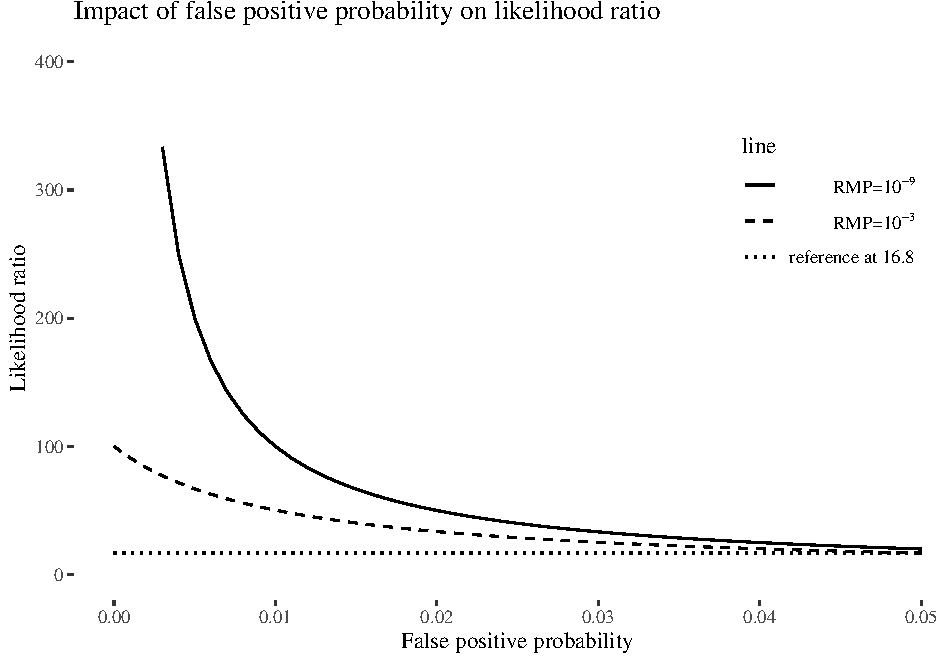
\includegraphics[width=0.7\linewidth]{lr-chapter3_files/figure-latex/unnamed-chunk-2-1} \end{center}
\caption{Dependencies between variables in the false positive problem.}
\label{fig:fpp}
\end{figure}

The formula we will end up with is:

\begin{align}
\tag{FPP-LR} \mathsf{LR}(R, S, \n S) & = \frac{1}{RMP + [ FPP \times (1-RMP)]}
\end{align}

\noindent where RMP stands for the random match probability and FPP for
the false positive probability. Re-written in terms of explicit
probabities the formula reads:

\begin{align*}
\mathsf{LR}(R,S, \n S) & = \frac{1}
{\pr{R \vert  M}\pr{ M \vert \n S} + \pr{R \vert \n M}\pr{\n M \vert \n S}}
\end{align*}

\noindent The denominator mirrors the fact that there are two ways
misleading evidence can arise: there is a true match and the suspect is
not the source (so it's a random match), or there is no real match, and
an error has been made in the identification process.

We will assume that whether a (lack of) match is reported is independent
of whether it is coincidental,

\begin{align}
\label{eq:indOnS}
\pr{R \vert M \et S} & = \pr{R \vert M \et \n S} = \pr{R \vert M}
\\ \nonumber
\pr{R \vert \n M \et S} & = \pr{R \vert\n M \et \n S} = \pr{R \vert \n M},
\end{align}

\noindent  that the probability of true match if the suspect is a source
is 1,

\begin{align}
\label{eq:ifSthenM}
\pr{M\vert S} = 1  \,\,\, \mbox{ so also } \,\,\, \pr{\n M \vert S}=0,
\end{align}

\noindent and that the probability that a true match is reported,

\begin{align}
\label{eq:fnNull}
\pr{R \vert M} & = 1.
\end{align}

Here, for simplicity we take the probability of a false negative to be
null; in fact, some of the reasons for taking false positives seriously
are also reasons to take false negatives seriously, but let's deal with
one problem at a time (and in the end, the impact of a false positive
risk will be clear from the way the formula will be derived). Now, let
us rewrite the numerator of the LR by extending the conversation,
rewriting the probabilities of conjunctions in terms of conditional
probability and simplifying:

\begin{align}
\label{eq:numer}
\pr{R\vert S} & = \frac{\pr{R\et S}}{\pr{S}} \\ \nonumber
& = \frac{\pr{R \et M \et S} + \pr{R \et \n M \et S}}
{\pr{S}}  \\ \nonumber
& = \frac{\pr{R \vert M \et S}\pr{M \vert S}\pr{S} + \pr{R \vert \n M \et S}\pr{\n M \vert S}\pr{S}}
{\pr{S}}  \\ \nonumber 
& = \pr{R \vert M \et S}\pr{M \vert S} + \pr{R \vert \n M \et S}\pr{\n M \vert S}
\end{align}

\noindent  Analogously, we can rewrite the denominator:

\begin{align}
\label{eq:denom}
\pr{R \vert \n S} & = \pr{R \vert M \et \n S}\pr{M \vert \n S} +
\pr{R \vert \n M \et \n S}\pr{\n M \vert \n S}
\end{align}

Putting \eqref{eq:numer} and \eqref{eq:denom} together, we have that:

\begin{align}
\label{eq:LRfp1}
\mathsf{LR}(R,S, \n S) & = \frac{\pr{R \vert M \et S}\pr{M \vert S} + \pr{R \vert \n M \et S}\pr{\n M \vert S}}
{\pr{R \vert M \et \n S}\pr{M \vert \n S} +
\pr{R \vert \n M \et \n S}\pr{\n M \vert \n S}}
\end{align}

Now, apply \eqref{eq:indOnS} in four places:

\begin{align}
\label{eq:LRfp2}
\mathsf{LR}(R,S, \n S) & = \frac{
\pr{R \vert M}\pr{M \vert S} + \pr{R \vert \n M}\pr{\n M \vert S}
}{
\pr{R \vert M }\pr{M \vert \n S} +
\pr{R \vert \n M}\pr{\n M \vert \n S}
}
\end{align}

Then, use \eqref{eq:ifSthenM} in the numerator:

\begin{align}
\label{eq:LRfp3}
\mathsf{LR}(R,S, \n S) & = \frac{
\pr{R \vert M} \times 1 + \pr{R \vert \n M}\times 0
}{
\pr{R \vert M }\pr{M \vert \n S} +
\pr{R \vert \n M}\pr{\n M \vert \n S}
}
\end{align}

Finally, \eqref{eq:fnNull} yields:

\begin{align}
\label{eq:LRfp4}
\mathsf{LR}(R,S, \n S) & = \frac{1}
{\pr{R \vert  M}\pr{ M \vert \n S} + \pr{R \vert \n M}\pr{\n M \vert \n S}}
\end{align}

Once we abbreviate \(\pr{M\vert \n S}\) as RMP, \(\pr{R \vert \n M}\) as
FPP and \(\pr{\n M \vert \n S}\), we arrive at the desired formula.

In Figure \ref{fig:fpplr} we illustrate this impact for the range of FPP
between 0 and 0.05, for two values of RMP: \(10^{-9}\) (often reported
in the case of two single-source samples over ten or more loci) and
\(10{^-3}\) (sometimes obtained by means of less discriminating tests
when the comparison involves a mixed sample). The upshot is that even a
small increase in FPP can lower the likelihood ratio dramatically, which
is yet another reason not to ignore FPP in DNA evidence evaluation. In
our illustration, we look at two pieces of DNA evidence with the two RMP
rates at \(1*10^8\) and \(100\), respectively. If the false positive
probability reaches 0.02, they fall down to \(\approx 49.99\) and
\(\approx 33.55\), and they get fairly close to each other already at
\(FPP=0.05\), where they are \(\approx 20\) and \(\approx 16.8\).

\begin{figure}

\begin{center}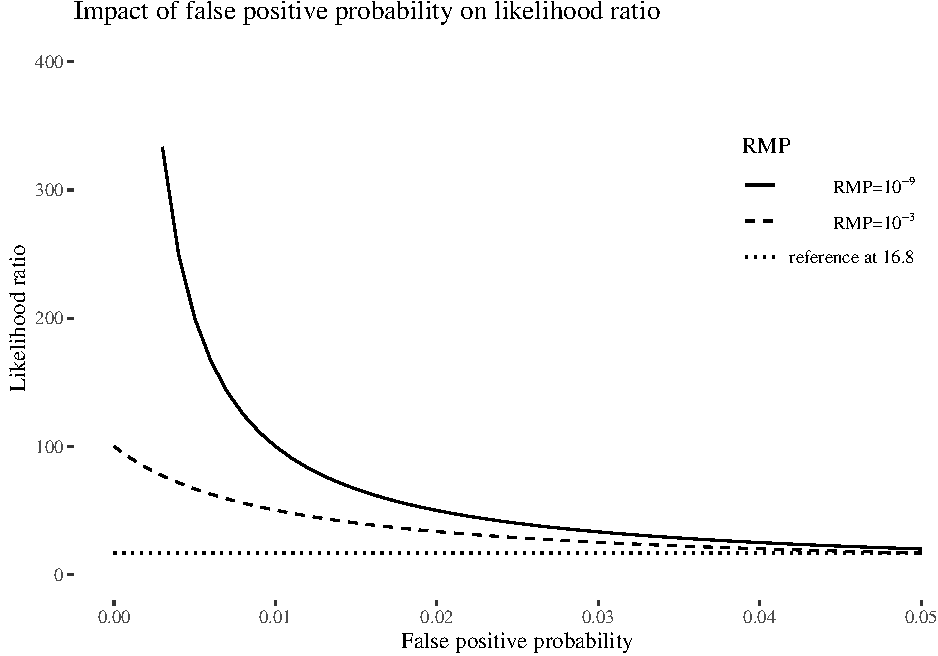
\includegraphics[width=1\linewidth]{lr-chapter3_files/figure-latex/fig-fpplr-1} \end{center}
\label{fig:fpplr}
\caption{Impact of the false positive probability on the likelihood ratio for two values of RMP. The horizontal reference line is at 16.8, the likelihood reached at RMP=$10{^-3}$ for FPP=0.05. At the same value of FPP, the LR for RMP $10{^-9}$ is 20.}
\end{figure}

\todo{M: I wonder if there is a deeper point here. That is, extremely low RMP values are meaningless when they cannot be accompanied by equally low FPP. See Alex's comment via email.}

Interestingly, Buckleton, Bright, \& Taylor (2018) give a seemingly
different formula for the impact of errors on likelihood ratio. Since
the derivation is simpler and it turns out that in fact this is simply a
more general formula, of which (FPP-LR) is just a particular instance,
it worth taking a look.

First, Buckleton et al. (2018) make the conceptual distinction between
the probability that an error occurs (\(E\)) and the probability that a
match is reported if it
does.\todo{Added worning, I can rewrite the proof if you can think of a better abbreviation.}
Mind your head: here \(E\) stands for error, not for evidence! In terms
of our notation, we have:

\begin{align*}
e & = \pr{E} = \pr{E \vert S} = \pr{E \vert \n S}
\end{align*}

\noindent That is, we denote the probability of error as \(e\), and we
assume it doesn't depend on whether the prosecution hypothesis is true
(whether the suspect is the source).

Separately, the formula includes the probability of a reported match if
an error occurs, also assumed to be independent of whether the
prosecution hypothesis is true:

\begin{align*}
k =  \pr{R \vert E, S} = \pr{R \vert E, \n S}
\end{align*}

\noindent Further, it is assumed that the probability of false negatives
is zero (\(\pr{R \vert S, \n E} =1\)) and the probability of reported
match if no error occurs and the defense hypothesis is true is RMP
(\(\pr{R \vert \n E, \n S}=RMP\)).

Now the derivation:

\begin{align*}
LR & = \frac{\pr{R\vert S}}
{\pr{R \vert \n S}}\\
& = \frac{\pr{R \vert \n E, S}\pr{\n E \vert S} + \pr{R \vert E, S}\pr{E \vert S}}
{\pr{R \vert \n E, \n S}\pr {\n E \vert \n S} + \pr{R \vert E, \n S}\pr{E \vert \n S}}\\
& = \frac{1(1-e) + ke}
{RMP(1-e)+ke}  = \frac{1-e+ke}{RMP  - e\times RMP + ke} \\
& = \frac{1 - (1-k)e}{RMP(1-e)+ke}
\end{align*}

\todo{I added these three passages to explain the argument, is this clear now?}
Let's take it slow. First, the likelihood ratio is just the ratio of
probabilities of a reported match (1) if the suspect is the source and
(2) if the suspect is not the source.

Now, think of \(\pr{R\vert S}\). This can be split into two possible
scenarios: an error has not been made, or an error has been made.
Accordingly, the numerator in the second line uses the law of total
probability to split \(\pr{R\vert S}\) into these two options.

Similarly, \(\pr{R\vert \n S}\) can be split into two cases: the suspect
is not the source, but we are dealing with a random match, or the
suspect is not the source, and an error has been made. An application of
the law of total probability in the denominator mirrors this. The rest
of the argument is just rewriting in terms of abbreviations, and
algebraic manipulation.

Note now that if you think of an error as something that guarantees a
mistaken identification, \(k\) becomes \(1\) and \(e\) becomes the false
positive rate. On this assumption straightforward algebraic manipulation
gives:

\begin{align*}
 \frac{1 - (1-k)e}{RMP(1-e)+ke} & = \frac{1-e+e}{RMP(1-e)+e}\\
 & = \frac{1}{RMP - e\times RMP + e} = \frac{1}{1 + e(1-RMP)}
\end{align*}

\noindent which is the same as the formula obtained by Aitken et al.
(2003) if we take \(e\) to be FPP, as we should on the assumption that
\(k=1\).

\todo{Do you also want me to explain the manipulation here?}

An analogous reasoning can be used to study the impact of false negative
probability on the value of exculpator DNA evidence. Consider the
probability of no match being reported if an error has been made,
anaologus to \(k\) above:

\begin{align*}
l & = \pr{\n R \vert E, S} = \pr{\n R \vert E, \n S} = \pr{\n R\vert E}
\end{align*}

\noindent Now, the likelihood ratio calculations, assuming \(l = 1\), go
as follows:

\begin{align*}
\mathsf{LR}(\n R, S, \n S) & = \frac{\pr{\n R \vert S}}{\pr{\n R \vert \n S}} \\
& = \frac{\pr{\n R \vert \n E, S}\pr{\n E \vert S} + \pr{\n R \vert E, S}\pr{E \vert S}}
{\pr{\n R \vert \n E, \n S}\pr{\n E \vert \n S} + \pr{\n R \vert E,\n S}\pr{E \vert \n S}} \\
& = \frac{0 (1-e) +  le}
{(1-RMP)(1-e) + le} \\
& = \frac{le}
{1- RMP - e + eRMP + le} = \frac{le}{1-RMP + e(l + RMP -1)}\\
& = \frac{e}{1 - RMP + eRMP} = \frac{e}{1+(e-1)RMP}
\end{align*}

\todo{Now, this argument is very similar, do we really need an informal gloss here as well?}

\noindent If the error rate is 0, then the numerator is 0 and so is the
\textsf{LR}, as it should. In such a case, the evidence is completely
exculpatory, the posterior probability that the suspect is the source
will be also 0. If the error rate is not 0, the numerator simply is the
probability of error, and the numerator takes values between \(1-RMP\)
and \(1\), depending on the value of \(e\). Quite crucially, 1 in the
denominator is decreased by \((1-e)RMP\), which with usually very low
RMP in the case of DNA evidence is a very small change as compared to
one, so the denominator stays very close to 1 even if \(e\) is very
high, and the \textsf{LR} effectively simply is
\(\approx \nicefrac{e}{1} = e\). The lines in Figure \ref{fig:fnplr},
strictly speaking, do not overlap, but the difference between them (with
\(RMP\) being fairly low) is negligible.

\begin{figure}

\begin{center}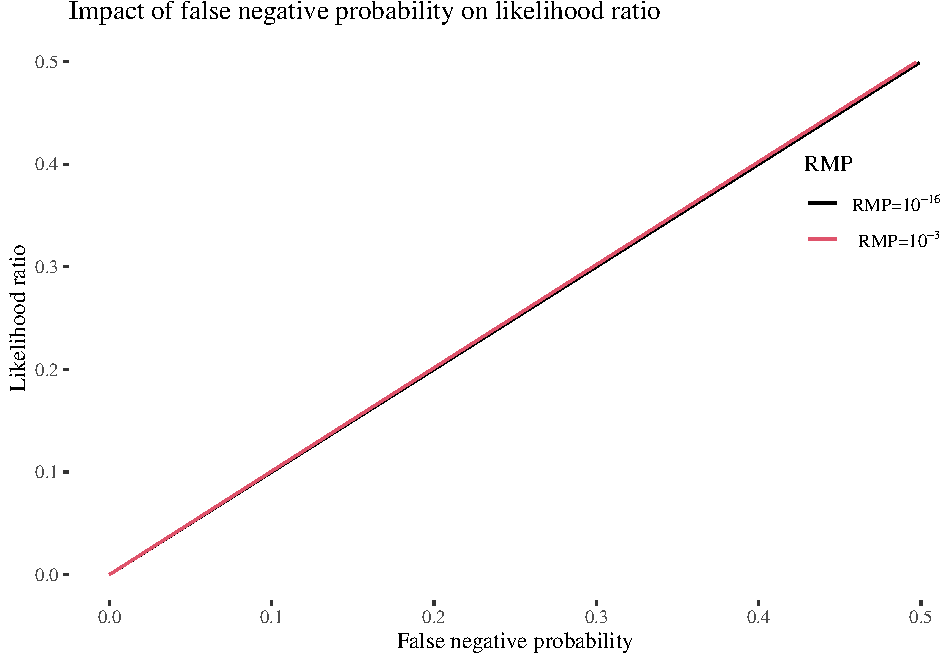
\includegraphics[width=1\linewidth]{lr-chapter3_files/figure-latex/fig-fnplr-1} \end{center}
\label{fig:fnplr}
\caption{Impact of the false negative probability on the likelihood ratio of exculpatory evidence for two values of RMP.}
\end{figure}

Interestingly, there is a sense in which the situation is not symmetric
when we compare FPP to FNP. With FPP, the LR is 50 when \(e=0.01\) for
RMP\(=10^{-3}\), while for the same \(e\) and RMP it is \(0.01\) for
FNP, an hundredfold decrease. This illustrates that the exculpatory
value of DNA evidence is higher than its incriminating value, even if
the error rates and random match probabilities are the same.

Some conceptual symmetry can be regained though. Suppose \(RMP\) is
really low as compared to \(FPP\) and let's ignore it in our
approximation. Then, the likelihood ratio of the incriminating evidence
becomes \(\nicefrac{1}{FPP}\) and the likelihood ratio of exculpatory
evidence becomes \(\nicefrac{FNP}{1}\). However, the change rate of
these differ. While
\(\nicefrac{d}{dx}(\nicefrac{1}{x}) = \nicefrac{d}{dx} (x^{-1}) = - \nicefrac{1}{x^2}\),
\(\nicefrac{d}{dx}(\nicefrac{x}{1})=1\), and the derivatives look quite
different (Figure \ref{fig:der})

\begin{figure}[h]

\begin{center}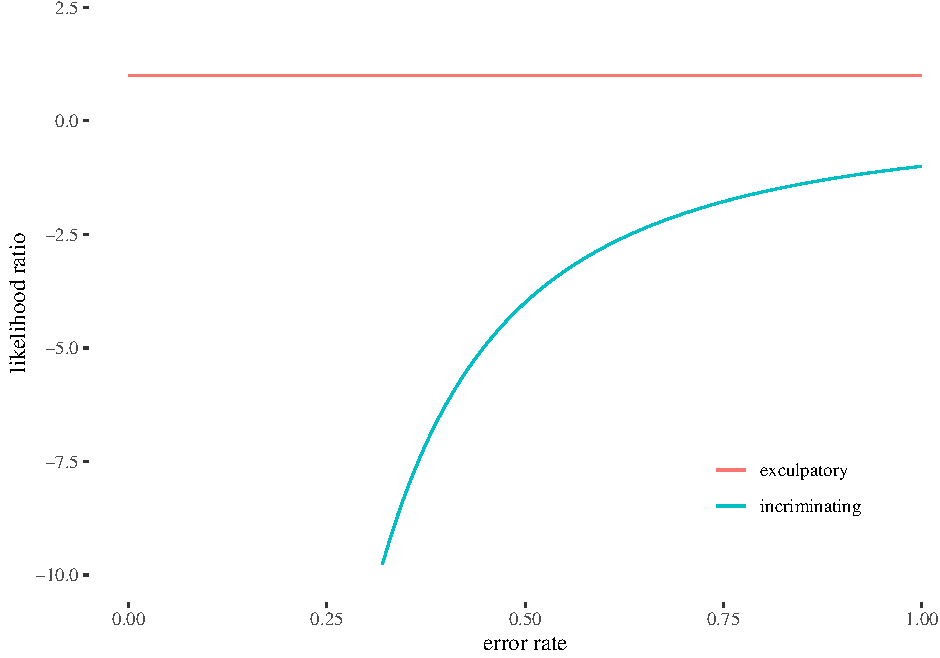
\includegraphics[width=1\linewidth]{lr-chapter3_files/figure-latex/unnamed-chunk-3-1} \end{center}
\caption{Derivatives of incriminatory and exculpatory likelihood ratios, range restricted to (-10,2).}
\label{fig:der}
\end{figure}

\todo{Added some explanation of the apparent assymetry does this help?}

\todo{Added this summary passage here, let me know what you think} The
key lesson from this section is as follows. First, likelihood ratios are
useful in the evaluation and comparison of the impact of positive an
negative error rates: and it makes clear that this impact is not the
same, contrary to what one may intuitively think. Second, the likelihood
ratio analysis reveals that even a seemingly small error rate in a sense
trumps random match probability: if you think there are good reasons to
worry about random matches, the analysis shows that there are much
better reasons to worry about error rates.

\section{\texorpdfstring{Eyewitness identification and likelihood ratio
\label{sec:eyewitness}}{Eyewitness identification and likelihood ratio }}\label{eyewitness-identification-and-likelihood-ratio}

So far we paid attention to DNA evidence, which rather uncontroversially
is quantitative. This might give the impression that likelihood ratio is
useful only for thinking about clearly quantitative evidence of this
sort. In this section, we discuss how likelihood ratio is still useful
for reflecting on evidence which, at leat seemingly, is not
quantitative: eyewitness evidence and for combining various items of
evidence.

We will argue that a quantitative perspective on eyewitness evidence is
not only available, but also useful. First, it teaches us that intuitive
evaluation of such evidence leads us astray more often than we tend to
think. Second, it provides us with better tools of eyewitness evidence
evaluation, as it allows us to study factors that impact its
reliability. Next, we will sketch how such a quantitative perspective
clears the path to a likelihood ratio treatment of such evidence: (i) in
likelihood ratio evaluation of a stand-alone piece of eyewitness
evidence, (ii) in combination of eyewitness evidence with a piece of
quantitative incriminating evidence, and (iii) in adjudication when
different pieces of evidence collide.

The perspective we take here is that there is no magical barrier between
quantitative and qualitative evidence. A certain type of evidence can
become numerical if sufficient amount of evidence about its reliability
has been collected and statistically analyzed. Eyewitness testimony is
not only no exception, but also a good example of this. We will now go
over the main quantitative findings regarding the reliability of
eyewitness evidence. Next, we will show how insights from such findings
can be used in a likelihood ratio analysis of the impact of eyewitness
evidence.

First of all, quantitative analyses might lead to a more sensible
assessment of evidence than merely intuitive judgments. In the case of
eyewitness testimony, this is crucial because eyewitness evidence tends
to be overvalued, and it is the quantitative information that can and
should be used to stop this madness. Field studies indicate filler
identification rates of 20-24\% (Klobuchar, Steblay, \& Caligiuri, 2006)
in eyewitness identifications. That is, around 20\% of the time, an
innocent presented to an eyewitness is going to be `identified' by the
eyewitness (the situation is a bit more complicated, read on for
details).

To get a better perspective on the fallibility of eyewitness evidence,
consider that 4.1\% is a conservative estimate of false death sentence
convictions in the United States, and those are based on much stronger
and multiple pieces of evidence, not a single eyewitness' testimony
(Gross, O'Brien, Hu, \& Kennedy, 2014). A study of 340 exonerations in
years 1989-2003 indicates that around 90\% of false convictions for rape
(and pretty much all inter-racial rape mistaken convictions) are based
on eyewitness misidentification, and that in 43\% of false convictions
for murder the defendant was misidentified by one or more eyewitnesses.

What else is quantitatively known about the reliability of eyewitness
testimony? A study of line-ups in 1561 witnesses and 616 suspect in real
cases in Greater London (Wright \& McDaid, 1996) and of 689
identification attempts in 271 real identification cases in Sacramento
(Behrman \& Davey, 2001) suggest false positive rate of around 20\%.
Also in experimental setting (where the witnesses are less emotionally
affected by the crime), eyewitnesses identify a filler in approximately
twenty percent of all real criminal line-ups (Thompson, 2007).

Moreover, studies of cross-examination failed to show that it improves
accuracy and that there is a clear relation between witness' confidence
and accuracy. In a series of experiments subjects were asked to
cross-examine eyewitnesses to determine whether witnesses made accurate
or mistaken identifications. Subjects have shown little or no ability to
make such discriminations (Wells \& Olson, 2003). Another example of the
unreliability of cross-examination is an experiment by Lindsay, Wells,
\& Rumpel (1981), in which a representative sample of \(48\) witnesses
was cross-examined. Subjects (\(n = 96\)) viewing the cross-examinations
showed no ability to distinguish accurate- from false-identification
witnesses within conditions as measured by subjects' trust in witnesses.

Moreover, there are various factors that have impact on the reliability
of eyewitness testimony, and here is where the quantitative analysis
shines. Several of the eyewitness quality issues have been studied by
means of experimental methods. Some of them are systemic variables
(simultaneous/sequential lineups,
showups,\footnote{Two basic types of identification procedures can be found in the literature, lineups, and field showups. A showup refers to the observation of a single suspect by a witness in the field, typically at the crime scene, whereas a lineup refers to the presentation of the suspect and several foils, either live or via photographs.}
presence of prior identification, culprit present/culprit absent,
frequency of witnesses per suspect), some of them---estimator variables
-- are not (the effect of delay, cross versus own-race effects, weapon
focus effects, presence of violence)---see (Behrman \& Davey, 2001) and
(Wells \& Olson, 2003) for an interesting discussion of such factors.

A fascinating meta-analysis by Wixted \& Wells (2017) suggests an even
more complicated picture, whose key points are as follows:

\begin{itemize}
\item
  In light of the empirical results that we've discussed and results
  similar to them the justice systems has grown more suspicious of
  eyewitness evidence over the last twenty years or so, especially
  doubting whether the eyewitness confidence is predictive of accuracy.
\item
  Isolating cases in which the identification has been made
  \emph{in pristine conditions} with high \emph{initial} confidence
  focusing on cases which would go to trial, that is, in which the
  suspect indeed was identified with high confidence, Wixted \& Wells
  (2017) argue that the data show that in such circumstances, the
  eyewitness confidence indeed is highly predictive of accuracy.
\item
  Pristine conditions involve a double-blind experiment containing only
  one suspect, at least five fillers, with no fillers who don't look
  like the perpertator at all, from among which the suspect doesn't
  stand out as obviously fitting the description which the eyewitness is
  familiar with, with no extreme coincidental resemblance of a filler to
  the suspect. The witness has to be cautioned that the offender might
  not be in the line-up and understand that they aren't failing if they
  don't indicate anyone, and the confidence statement needs to be
  collected at the time of first identification. Very few police
  departments are known to run their lineups in pristine conditions.
\item
  Whether the conditions were pristine and whether the eyewitness
  initial confidence was high are factors which trump the role of the
  estimator variables.
\item
  The extent to which initial high confidence in pristine conditions is
  predictive of identification accuracy depends on the base rate of
  target-present lineups. In lab studies it is usually fixed at around
  50\%, but it is expected to vary widely in real circumstances. The
  best estimate is around 35\%, and it seems that at that base rate
  high-confidence witnesses (initial confidence, pristine conditions)
  are around 90\% accurate.
\item
  With time, and especially in the contexts in which a witness expects a
  cross-examination, witness confidence loses its predictive power.
  Preparations for the trial are known to inflate witness confidence,
  especially if they received a positive feedback from anyone after the
  initial identification.
\end{itemize}

Ideally, properly formatted data about all the factors we disussed
could, with appropriate effort, be used to develop a multivariate model
which would lead to quantitative eyewitness reliability estimates,
including some estimation of the uncertainty involved. While we are far
from reaching the state of such maturity, it should be clear that even
with the current state of knowledge, and expert in eyewitness testimony
evaluation aware of the literature some of which we have cited, aware of
the circumstances of the case and identification could express their
evaluation of the witness' reliability quantitatively. Claiming that an
untrained jury member can do better by just intuitively evaluating what
the eyewitness said instead is at least hasty.

So consider two scenarios in which we numerically estimate the
reliability of the eyewitness evidence in line with the research we just
discussed. In one, such an expert recognizes the identification
conditions as pristine and testifies: the probability of the testimony
if the suspect in fact is the perpetrator (\(\pr{E\vert H}\)) is
\(.9\% \pm .05\), and the false positive probability
(\(\pr{E \vert \n H}\)) is \(.1\pm .03\). In scenario two, the
conditions were not pristine, and the expert testifies that
\(\pr{E\vert H}=.8 \pm .05\) and \(\pr{E\vert \n H}=.25 \pm .05\). We
get two different \emph{ranges} of likelihood ratios, \(lr_1\) and
\(lr_2\). In the first case, the minimum and the maximum are as follows:

\begin{align*}
\mathsf{min}(lr_1) = \nicefrac{.95}{.07} \approx 13.57  & \,\,\,\,\,\,\,\,  \mathsf{max}(lr_1) = \nicefrac{.85}{.13} \approx 6.53  
\end{align*}

\noindent so the expert can, say, testify that the likelihood ratio is
in the range of 6.5-13.5. In the second scenario, the minimum and the
maximum are as follows:

\begin{align*}
\mathsf{min}(lr_1) = \nicefrac{.85}{.2} =  4.25 &  \,\,\,\,\,\,\,\,   \mathsf{max}(lr_1) = \nicefrac{.75}{.3} \approx 2.5  
\end{align*}

\noindent so the expert can testify that the likelihood ratio is in the
range of 2.5-4.25.

Now, suppose further evidence is put forward to the effect that the
suspect blood type matches the crime scene sample. Say the probability
of a match if the suspect is the source is simply 1, while the
probability of a random match is .05. The likelihood of this evidence
alone is \(\nicefrac{1}{.05}= 20\). Assuming indepedence, the joint
likelihood for total evidence is obtained by multiplying separate
likelihood ratios. Now, without any commitment to the priors, the impact
of likelihood ratio ranges on any prior probability can be quantified
and visualised, as in Figure \ref{fig:eyewitness3}.

\begin{figure}[h]

\begin{center}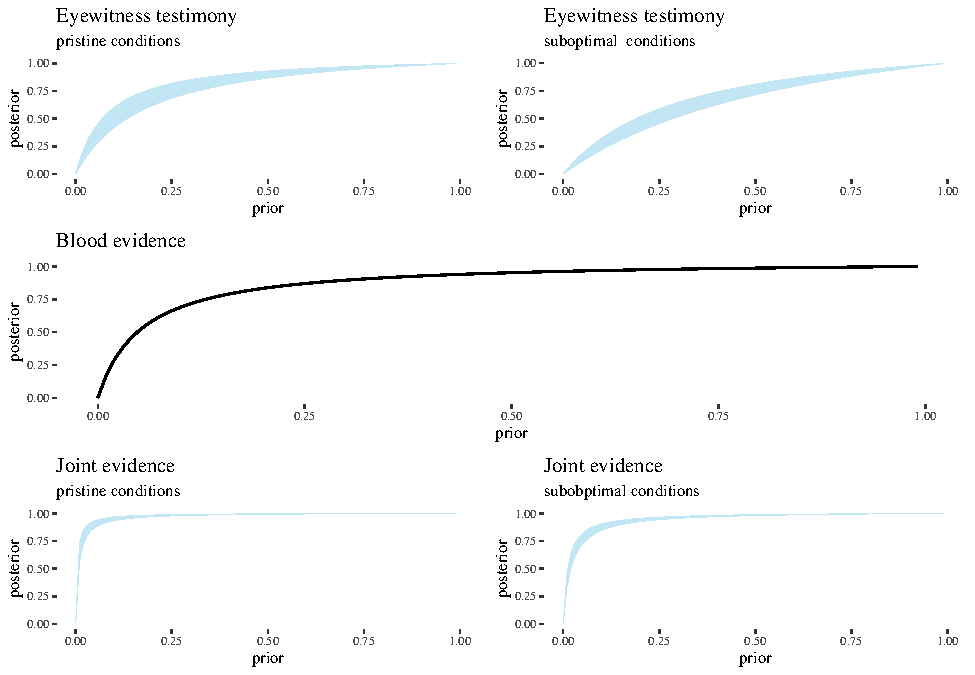
\includegraphics[width=1\linewidth]{lr-chapter3_files/figure-latex/eyewitness2-1} \end{center}
\caption{Impact of converging items of  evidence on the posteriors.}
\label{fig:eyewitness3}
\end{figure}

What about conflicting evidence? Suppose this time the conditions were
pristine, the expert's evaluation of the eyewitness evidence in pristine
conditions is as before, but the witness identified someone else than
the suspect (evidence \(E\)), while DNA evidence (evidence \(D\))
supports the prosecution hypothesis \(H\) with \textsf{LR} = 300 (this
is, say, because we take the false positive probability seriously).
Then, the range of plausible likelihood ratios for eyewitness evidence
alone is:

\begin{align*}
\left[\frac{.07}{.95}, \frac{.13}{.85}    \right ]  & \approx [.073,.15]
\end{align*}

In contrast, if the eyewitness is a friend of the suspect, so that you
estimate \(\pr{E \vert H}\) to be .6, while the conditions were
suboptimal, so that \(\pr{E\vert \n H} = .8\pm .05\), the likelihood
ratio range is \(.7-.8\) and the impact of such eyewitness evidence is
quite different.

\vspace{1mm} \footnotesize

\normalsize

\begin{figure}[h]

\begin{center}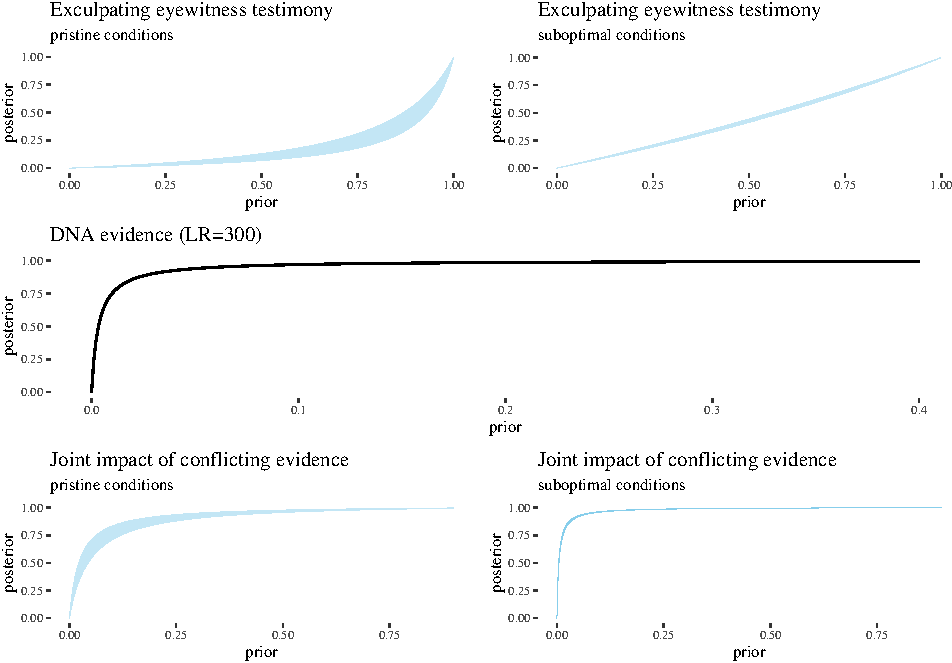
\includegraphics[width=1\linewidth]{lr-chapter3_files/figure-latex/eyewitness4-1} \end{center}
\caption{Impact of conflicting items of  evidence on the posteriors.}
\label{fig:eyewitness4}
\end{figure}

The key observation here is that whether exculpatory eyewitness
testimony can in fact be sufficient to acquit in light of incriminating
DNA evidence depends on the particulars: both on the quality of the
eyewitness testimony and on the realistic assessment of the likelihood
ratio for the DNA evidence (incorporating the probability of false
positives), and on what priors other pieces of evidence led us to so far
prior to the evaluation of such items of evidence. The devil is in the
detail, and it is not always the case that one should trump the other.

The reader might be disappointed: simply saying ``it depends'' does not
seem to help much. However, keep in mind that there are well known items
in the literature, on one hand, in psychology, illustrating that human
jurors tend to value eyewitness evidence over statistical evidence
(Niedermeier, Kerr, \& Messeé, 1999; Wells, 1992; Wells \& Olson, 2003),
and, on the other hand, in epistemology, attempting to explain this
intuition in a philosophically principled manner (Bolinger, 2020; Smith,
2017; Thomson,
1986).\todo{We might need more references in this passage, think about this.}
In line with a more balanced view (Redmayne, 2008), our approach
suggests that while the psychological effect exists, there are multiple
cases in which the preference for eyewitness evidence is mistaken, and
relegates the identification and evaluation of factors that contribute
to its proper evaluation to actual empirical research. If the situation
is complicated, the best that can be done is take its complexity
seriously, and quantitative methods are much more fit for this task than
juror's intuitions or general philosophical statements.

\vspace{3mm}
\textbf{I still need to take a look and discuss the  Rush decision}

\section{\texorpdfstring{Hypothesis choice
\label{sec:hchoice}}{Hypothesis choice }}\label{hypothesis-choice}

\todo{revised these two intro passages} The point so far is that the
likelihood ratio is a fruitful conceptual framework for assessing the
strength of the evidence. However, its use is not devoid of challenges,
and we move to a discussion of how they arise.

Now, we turn to a difficulty with the use of likelihood ratio in the
context of legal fact-finding: likelihood ratios is sensitive to the
hypothesis choice. We discuss this problem in general in this section,
(i) showing how an ad hoc hypothesis can always lead to a useless
likelihood ratio, (ii) discussing a real case in which the choice of
hypothesis was fairly confusing and had impact on evidence evaluation,
(iii) indicating that the problem doesn't arise if the hypotheses as
exclusive and exhaustive, and (iv) arguing that this theoretical
resolution may be unhelpful in practice, as there seem often to be good
reasons why experts do not use such pairs of hypotheses. Further, in
Section \ref{sec:lhTwoSTain} we further illustrate how large shifts in
the likelihood ratio can take place even if the hypotheses chosen seem
reasonable, and argue that another clear source of variability of
likelihood ratio is the choice of hypothesis levels. The two sections
taken together paint a difficulty with using likelihood ratio alone as a
measure of evidential strength and suggest that a more elaborate
framework, employing likelihood ratios, but not restricted to their
reporting, would be more useful.

One major difficulty, however, is the choice of the hypotheses \(H\) and
\(H'\) that should be compared. Generally speaking, the hypotheses
should in some sense compete with one another---say, in a criminal
trial, \(H\) is the hypothesis put forward by the prosecution and \(H'\)
is the hypothesis put forward by the defense. Presumably, the two
hypotheses should be something that the two parties disagree about. But
this minimal constraint offers too little guidance and leaves open the
possibility for manipulations and misinterpretations of the evidence.
What follows outlines some of the main arguments in the literature on
this topic.

Consider a stylized DNA evidence case. Suppose the prosecutor puts
forward the hypothesis that the suspect left the traces found at the
crime scene. This hypothesis is well supported by laboratory analyses
showing that the defendant genetically matches the traces.

The defense, however, responds by putting forward the following
\textit{ad hoc} hypothesis: `The crime stain was left by some unknown
person who happened to have the same genotype as the suspect.' Since the
probability of the DNA match given either hypothesis is 1, the
likelihood ratio equals 1 (Evett, Jackson, \& Lambert, 2000). The
problem generalizes. For any item of evidence and any given prosecutor's
hypothesis \(H\), there is an \textit{ad hoc} competing hypothesis
\(H^*\) such that \(\nicefrac{\pr{E \vert H}}{\pr{E \vert H^*}}=1\).

Hypothesis \(H^*\) is simply a just-so hypothesis, one that is selected
only because it explains the evidence just as well as hypothesis \(H\)
does (Mayo, 2018). If no further constraints are placed on the choice of
the competing hypotheses---it would seem---no evidence could ever
incriminate a defendant. This is unsettling.

One reply might be that this phenomenon need not be so damning in
practice. Judges and jurors, after all, will often recognize
\textit{ad hoc} hypotheses for what they are---artificial theories that
should not be taken seriously. Perhaps, the reasonable expectations of
the participants in a trial will suffice to constrain the choice of
hypotheses in just the right way.

One issue with this reply is that it is not principled. Fair enough,
maybe in practice fact-finders will avoid ad-hoc hypotheses. But why
should they avoid them, other than because otherwise the resulting
likelihood ratio will be useless? Moreover, as we will soon see,
hypothesis choice has impact on likelihood ratio even if no ad hoc
hypothesis seems to be used. Moreover, real cases tend to be quite
complex, and it is not always obvious whether a certain choice of
competing hypotheses, none of which are is obviously \textit{ad hoc}, is
legitimate or not. In what follows we will illustrate some of these
issues, and argue that due to this sensitivty, likelihood ratio alone is
not informative enough, if not supplied by careful considerations of
hypothesis choice.

Here is an example that illustrates how even when the competing
hypotheses are not obviously \textit{ad hoc}, the absence of a clear
rationale for their choice may create confusions in the assessment of
the evidence. In R.~v.~Barry George (2007 EWCA Crim 2722). Barry George
was accused of murdering TV celebrity Jill Dando. A key piece of
evidence at play was: \vspace{2mm}

\begin{center}
\begin{tabular}{lp{12cm}} 
    $E$ &  
    A single particle of firearm  residue (FDR) 
     was found one year later in George's coat pocket and it matched the residue from the crime scene.
     This was the key incriminating evidence against him. 
\end{tabular}
\end{center}

\vspace{2mm} \noindent  The defense argued that, since it was only one
particle, there must have been contamination. The experts for the
prosecution, however, testified that it was not unusual that a single
particle would be found on the person who fired the gun. George was
convicted, and his first appeal was unsuccessful.

After the first appeal, Dr.~Evett from the Forensic Science Service
worried that the evidence had not been properly assessed at trial. The
jurors were presented with the conditional probability
\(\pr{\textsf{residue}\vert H_d}\) of finding the firearm residue in
George's coat given the defense hypothesis \(H_d\) that George
\textit{did not} fire the gun. This probability was estimated to be
quite low, indicating that the evidence spoke against the defense's
hypothesis. But the jurors were not presented with the conditional
probability \(\pr{\textsf{residue}\vert H_p}\) of finding the same
evidence given the prosecutor's hypothesis \(H_p\) that George
\textit{did} fire the gun that shot Dando. An expert witness,
Mr.~Keeley, was asked to provide both conditional probabilities and
estimated them to be \(\nicefrac{1}{100}\), which indicated that the
firearm residue had no probative value. After new guidelines for
reporting low level FDR in 2006, the FSS re-assessed the evidence and
concluded that it was irrelevant. George appealed again in 2007, and
relying on Keely's estimates, won the appeal.

At first, this case seems a good illustration of how likelihood ratios
help to correctly asses the value of the evidence presented at trial.
But this reading of the case would be overly optimistic. In fact, a
close study of the trial transcript shows that Keeley's choice of
hypotheses was not systematic and the likelihood ratio based on them was
therefore really hard to interpret (Fenton, Berger, Lagnado, Neil, \&
Hsu, 2014). For instance, Mr Keeley is reported to have said:

\begin{quote}
    It was necessary to balance the likelihood that the particle came from a gun fired by the appellant and the likelihood that it came from some other source. Both were unlikely but both were possible.
\end{quote}

\noindent  Keeley compared the hypothesis that the particle found in
George's pocket came from a gun fired by George himself, and the
alternative hypothesis that the particle came from another source. In
line with the quotation, Keeley said that the prior probabilities of
both hypotheses should be low. But this is mathematically impossible if
they were exhaustive and exclusive.

On another occasion, Keeley took the prosecutor's hypothesis to be `The
particle found in George's pocket came from the gun that killed Dando'
and the defense hypothesis to be `The particle on George's pocket was
inserted by contamination.' The problem is that the evidence is a
logical consequence of either of them, so the conditional probability of
the evidence given each of these hypothesis is one. Crucially, they are
therefore useless for the evaluation of the weight of evidence, because
in such case the likelihood ratio will always be one for trivial
reasons. The most charitable reading of the trial transcript suggests
that the expert had in mind the hypotheses `George was the man who shot
Dando' and `The integrity of George's coat was corrupted.' But these
hypotheses are neither exhaustive nor exclusive, and Keeley gave no
clear criterion for why these hypotheses should be compared in the
likelihood ratio (see Fenton et al., 2014 for further details).

The confusion in the Barry George case is attributable to the absence of
clear rules for choosing the hypotheses in the likelihood ratio. One
such rule could be: pick competing hypotheses that are exclusive (they
cannot be both true) and exhaustive (they cannot be both false). In this
way, the parties would not be able to pick \textit{ad hoc} hypotheses
and skew the assessment of the evidence in their own favor.

Besides blocking partisan interpretations of the evidence, there are
other principled reasons to follow the exclusive-and-exhaustive rule,
specifically, the fact that when the hypotheses are not exclusive or
exhaustive, the likelihood ratio might deliver counterintuitive results
and cause confusion in the assessment of the strength of the evidence.
If two competing hypotheses, \(H_p\) and \(H_d\) are not mutually
exclusive, it is possible that they both make the evidence equally
likely (the likelihood ratio is one), and yet the posterior
probabilities of the hypotheses given the evidence are higher than their
prior probabilities.

For instance, let \(H_p\) stand for `The defendant is guilty' and
\(H_d\) for `The defendant was not at the crime scene'. Both hypotheses
might be true. Let \(E\) stand for `Ten minutes before the crime took
place the defendant---seen at a different location--- was overheard on
the phone saying \emph{go ahead and kill him}.' It is conceivable that
the likelihood ratio should equal one in this context, yet the posterior
probabilities of each hypothesis, given \(E\), should be higher than the
prior probability. So, intuitively, the evidence should positively
support each hypothesis, contrary to what the likelihood ratio would
suggest.

Further, when the two competing hypotheses are not exhaustive, the
likelihood ratio may once again clash with our intuitions. The
likelihood ratio might then equal one even though the evidence lowers
their posterior probability. For example, suppose Fred and Bill
attempted to rob a man. The victim resisted, was struck on the head and
died. Say \(H_p\) stand for `Fred struck the fatal blow' and \(H_d\)
stand for `Bill struck the fatal blow.' The hypotheses are not
exhaustive. A missing hypothesis is `The man did not die from the blow.'
Suppose \(E\) is the information that the victim had a heart attack six
months earlier. The likelihood ratio
\(\nicefrac{\pr{E \vert H_p}}{\pr{E \vert H_d}}\) equals one since
\(\pr{E\vert H_p}=\pr{E\vert H_d}\). Yet \(E\) reduces the probability
of both \(H_p\) and \(H_d\). So, in this case, the evidence should
negatively support each hypothesis, contrary to what the likelihood
ratio suggests.\\
Whether the exhaustive-and-exclusive rule would be a good guiding
principle, however, is not clear-cut. Requiring that the hypotheses be
always exclusive and exhaustive hypotheses is not without complications
either. For consider an expert who decides to formulate the defense
hypothesis by negating the prosecution hypothesis, say, `the defendant
did not hit the victim in the head.' This choice of defense hypothesis
can be unhelpful in assessing the evidence, because the required
probabilities are hard to estimate. For instance, what is the
probability that the suspect would carry such and such blood stain if he
did not hit the victim in the head? This depends on whether he was
present at the scene, what he was doing at the time and many other
circumstances.

(Reader warning: this passage will discuss hypothesis choice in a rape
case.) Similarly, in a rape case, it is hard to estimate the probability
of the matching evidence if the suspect did not have the intercourse
with the victim. Instead, what is considered is the hypothesis that
someone else, unrelated to the suspect, had intercourse with the victim.
As (Evett et al., 2000) point out, in many real life rape cases the
choice of a particular hypothesis to be used by the expert in the
evaluation of the strength of the evidence (of, say, the lack of semen
in a rape case), will depend on contextual factors. Sometimes it will be
`intercourse did not take place,' sometimes it will be `the intercourse
took place, but the complainant used a vagina douche,' or sometimes
`another sexual act took place'. More often than not, the hypotheses
chosen will not be mutually exclusive.

Moreover, comparing exclusive and exhaustive hypotheses can also be
unhelpful for jurors or judges making a decision at trial. In a
paternity case, for example, the expert should not compare the
hypotheses `The accused is the father of the child' and its negation,
but rather, `The accused is the father of the child' and `The father of
the child is a man unrelated to the putative father' (Biedermann, Hicks,
Taroni, Champod, \& Aitken, 2014). The choice of the latter pair of
competing hypotheses is preferable. Even though the relatives of the
accused are potential fathers, considering such a far-fetched
possibility would make the assessment of the evidence more difficult
than needed. At the same time, if the defense hypothesis is too
specific, \textit{ad hoc} and entails the evidence, it won't be of much
use. For example, take `The crime stain was left by some unknown person
who happened to have the same genotype as the suspect.' The probability
of a DNA match given this hypothesis would be 1. But usually the
probability of the DNA match given the prosecution's hypothesis, say
`The crime stain was left by the suspect,' is also 1. This would result
in a rather uninformative likelihood ratio of 1. Another feature of such
specific explanations is that it's hard to reasonably estimate their
prior probability, and so hard to use them in arguments between opposing
sides. (Evett et al., 2000).

\todo{M: We should mention a dispute between Taroni research group and Fenton research group about LR. Is this in the references? They seem to disagree on this quite a bit. Bringing out the puzzle in their dispute could be philosophically very interesting even if we do not give a complete resolution.}

\todo{You keep mentioning this dispute, but I never got the impression of deep disagreement. Maybe I missed something, do you have any specific papers in mind?}

So, it seems, the choice of competing hypotheses lies between two
extremes. Exclusive and exhaustive hypotheses guard against ad hoc
hypotheses, arbitrary comparisons and ensure a more objective assessment
of the evidence. Unfortunately, exhaustive and exclusive hypothesis
cover the entire space of possibilities, and sifting through this space
may be cognitively unfeasible. So, in this respect, comparing more
circumscribed hypotheses is preferable. The danger of doing so, however,
is slipping into arbitrariness as likelihood ratios heavily depend on
the hypotheses that are compared. The more latitude in the choice of the
hypotheses, the more variable the likelihood ratio as a measure of
evidentiary value. This is a particularly troubling phenomenon, as
competing hypotheses can concern any factual dispute, from minute
details such as whether the cloth used to suffocate the victim was red
or blue, to ultimate questions such as whether the defendant stabbed the
victim.

To add another complication, the likelihood ratio varies across
hypotheses formulated at different levels of granularity: offense,
activity and source level hypotheses. It is even possible that, at the
source level, the likelihood ratio favors one side, say the prosecution,
but at the offence level, the likelihood ratio favors the other side,
say the defense, even though the hypotheses at the two levels are quite
similar. Further, a likelihood ratio that equals 1 when source level
hypotheses are compared may tip in favor of one side or the other when
offence level hypotheses are compared (Fenton et al., 2014). This
variability makes the likelihood ratio a seemingly arbitrary---and
easily manipulable---measure of evidentiary value.

The likelihood ratio can be misleading, but this risk is mitigated when
its assessment is accompanied by a careful discussion of a number of
issues, such as: which hypotheses are being compared; how they are
formulated; their level of granularity (that is, source, activity and
offense level); why the hypotheses are (or are not) exclusive and
exhaustive, and why other hypotheses are ruled out as unworthy of
consideration.

\todo{Added this summary passage, check.} This is our first warning sign
when it comes to relying on likelihood ratios. In real-life
applications, multiple hypotheses and pairs thereof are at play, and
their choice does matter. For this reason, merely reporting likelihood
ratios might be
misleading,\footnote{Similarly, BF would be sensitive to the choice of the prosecution hypothesis, but since BF faces other problems we already discussed, we will not get into this issue.}
and such a presentation of evidence is best accompanied by a careful
discussion of which hypotheses were considered, which were chosen and
why, and how they all are related to the evidence. Later on we will
argue that a clear treatment of such issues is immensely assisted by the
use of Bayesian networks in evidence presentation and evaluation. This
will be a recurring point in this book.

\section{\texorpdfstring{Levels of Hypotheses and the two-stain problem
\label{sec:lhTwoSTain}}{Levels of Hypotheses and the two-stain problem }}\label{levels-of-hypotheses-and-the-two-stain-problem}

\todo{added intro to improve flow} Since we want to put likelihood
ratios in their proper place when it comes to evidence evaluation and
reporting, we would like to obtain a deeper understanding of the factors
that might lead to their variation depending on the hypothesis choice.
let's take a closer look at one systematic dimension of hypothesis
choice sensitivity: likelihood ratios change with the levels of
hypothesis under consideration. In this section we take a closer look at
this issue.

To some approximation, hypotheses can be divided into three levels:
offence, activity, and source level hypotheses. At the offence level,
the issue is one of guilt or innocence, as in the statement `Smith
intentionally attacked the victim with a knife'. At the activity level,
hypotheses do not include information about intent but simply describe
what happened and what those involved did or did not do. An example of
activity level hypothesis is `Smith bled at the scene.' Finally, source
level hypotheses describe the source of the traces, such as `Smith left
the stains at the crime scene,' without specifying how the traces got
there. Overlooking differences in hypothesis level can lead to serious
confusions. To illustrate, consider a case in which a DNA match is the
primary incriminating evidence. In testifying about the DNA match at
trial, experts will often assess the probability that a random person,
unrelated to the crime, would coincidentally match the crime stain
profile\footnote{For a survey of developments and complications of this
  model, see (Foreman et al., 2003).} The random match probability is
often an impressively low number, say 1 in 100 million or lower, at
least excluding the possibility that relatives or identical twins would
coincidentally match (Donnelly, 1995). This should count as a strong
evidence against the suspect. But how exactly? RMP---the probability
that a random person from the population matches the crime stain
profile---is taken to be the probability that the suspect is a match if
in fact he is innocent and is usually estimated as the frequency of a
given profile in the relevant population. As we already know from the
chapter in which we discussed probabilistic fallacies \todo{crossref},
RMP is not the posterior probability of innocence, since
\(\pr{\textsf{match} \vert \textsf{innocence}}\) should not be confused
with \(\pr{\textsf{innocence} \vert \textsf{match}}\). To confuse the
two would be to commit the prosecutor's fallacy. Further, it is tempting
to equate the random match probability to
\(\pr{\textsf{match} \vert \textsf{innocence}}\) and together with the
prior \(\pr{\textsf{innocence}}\) use Bayes' theorem to calculate the
posterior probability of innocence
\(\pr{\textsf{innocence} \vert \textsf{match}}\). But this also might be
a mistake. Equating the random match probability with
\(\pr{\textsf{match} \vert \textsf{innocence}}\) overlooks the
difference between offense, activity and source level hypothesis. It is
hasty to assume that, in one way or another, a DNA match can speak
directly to the question of guilt or innocence. Even if the suspect
actually left the genetic material at the scene---source level
proposition---the match does not establish guilt. Even if the defendant
did visit the scene and came into contact with the victim, it does not
follow that he committed the crime he was accused of. It is true, that
in many circumstances the random match probability and the posterior
probability of innocence given a match would both be very low, but such
issues need to be considered and took into consideration in DNA evidence
evaluation.

Few forms of evidence can speak directly to offense level hypotheses.
Circumstantial evidence that is more amenable to a probabilistic
quantification, such as DNA matches and other trace evidence, does not.
Eyewitness testimony may speak more directly to offense level
hypotheses, but it is also less easily amenable to a probabilistic
quantification. This makes it difficult to assign probabilities to
offense level hypotheses. Experts are usually not supposed to comment
directly on offense level hypotheses, but they often comment on activity
level and source level hypotheses. In moving from source to activity
level, however, additional sources of uncertainty come into play. The
assessment of activity level hypotheses depends on additional variables
other than those on which the assessment of source level hypotheses
depends. For example, the probability of finding such and such quantity
of matching glass if the suspect smashed the window depends on how the
window was smashed, when it was smashed, and what the suspect did after
the action. Another problem arises due to recent improvements in DNA
profiling technology. Since today investigators are able to obtain
profiles from minimal amounts of genetic material, transfer
probabilities become more difficult to assess as more opportunities of
transfer arise. If small traces such as dust speckles can be used as
evidence, the possibility that the traces were brought to the scene
accidentally becomes more likely. For this reason, moving beyond source
level hypotheses requires a close collaboration between scientists,
investigators and attorneys (see Cook, Evett, Jackson, \& Jones, 1998
for a discussion). The choice and formulation of the hypotheses are up
for revision as new evidence is obtained or facts about what happened
are accepted (Evett et al., 2000). A case study that further illustrates
both advatanges and limitations of the likelihood ratio as a measure of
evidentiary strength is the two-stain problem, originally formulated by
Evett (1987). The key limitation is due to the combination of two
circumstances: first, that likelihood ratios vary depending on the
choice of hypotheses being compared; second, that it is not always clear
which hypotheses should be compared. To illustrate what is at stake,
what follows begins with Evett's original version of the two-stain
problem (which does not pose any challenge to the likelihood ratio) and
then turns to a more complex version (which suggests that likelihood
ratios, in and of themselves, are insufficiently informative). Suppose
two stains from two different sources were left at the crime scene, and
the suspect's blood matches one of them. More precisely, the two items
of evidence are as follows: \vspace{2mm}

\begin{center}
    \begin{tabular}{lp{10cm}} 
        $E_1$ & The blood stains at the crime scene are of types $\gamma_1$ and $\gamma_2$ of estimated  frequencies $q_1$ and $q_2$ respectively.\\
        $E_2$ & The suspect's blood type is $\gamma_1$. 
    \end{tabular}
 \end{center}

\vspace{2mm}

\noindent  Let the first hypothesis be that the suspect was one of the
two men who committed the crime and the second hypothesis the negation
of the first. \vspace{2mm}

\begin{center}
    \begin{tabular}{lp{12cm}} 
        $H_p$ & The suspect was one of the two men who committed the crime.\\
        $H_d$ & The suspect was not one of the two men who committed the crime.
    \end{tabular}
 \end{center}

\vspace{2mm} Evett (1987) shows that the likelihood ratio of the match
relative to these two hypotheses is \(\nicefrac{1}{2q_1}\) where \(q_1\)
is the estimated frequency of the characteristics of the first stain.
Surprisingly, the likelihood ratio does not depend on the frequency
associated with the second stain. To understand Evett's argument,
consider first the likelihood ratio:

\begin{align*}
\frac{\pr{E_1\wedge E_2\vert H_p}}{
    \pr{E_1\wedge E_2\vert H_d}} & = \frac{\pr{E_1 \vert E_2 \wedge H_p}}{
    \pr{E_1 \vert E_2 \wedge H_d}
    }\times 
 \frac{\pr{E_2\vert H_p}}{\pr{E_2 \vert H_d}}. 
 \end{align*}

\noindent Notice that the suspect's blood type as reported in \(E_2\) is
independent of whether or not he participated in the crime, that is,
\(\pr{E_2\vert H_p}=\pr{E_2 \vert H_d}\). So the likelihood reduces to:

\begin{align*}
 \frac{\pr{E_1\wedge E_2\vert H_p}}{
    \pr{E_1\wedge E_2\vert H_d}} & = \frac{\pr{E_1 \vert E_2 \wedge H_p}}{
    \pr{E_1 \vert E_2 \wedge H_d}.
 } 
 \end{align*}

\noindent
 The numerator \(\pr{E_1 \vert E_2 \wedge H_p}\) is the probability that
one of the stains is \(\gamma_1\) and the other \(\gamma_2\) given that
the suspect is guilty and has profile \(\gamma_1\). The probability that
one of the stains is \(\gamma_1\) is simply 1, and assuming blood type
does not affect someone's propensity to commit a crime, the probability
that the second stain is \(\gamma_2\) equals its relative frequency in
the population, \(q_2\). So the numerator is \(1\times q_2 = q_2\). \%
Next, consider the denominator \(\pr{E_1 \vert E_2 \wedge H_d}\). If
\(H_d\) is true, the fact that the suspect has profile \(\gamma_1\) is
irrelevant for the crime scene profiles. the crime was committed by two
randomly selected men with profiles \(\gamma_1\) and \(\gamma_2\), who
can be seen as two random samples from the general population as far as
their blood profiles are concerned. There are two ways of picking two
men with such profiles (\(\gamma_1,\gamma_2\) and
\(\gamma_2,\gamma_1\)), each having probability \(q_1q_2\). So the
denominator equals \(2q_1q\). By putting numerator and denominator
together, we have:

\begin{align*}
 \frac{q_2}{2q_1q_2} = \frac{1}{2q_1}. 
 \end{align*}

\noindent which completes the argument. In general, if there are \(n\)
bloodstains of different phenotypes, the likelihood ratio is
\(\nicefrac{1}{nq_1}\), or in other words, the likelihood ratio depends
on the number of stains but not on the frequency of the other
characteristics.

Consider now a more complex two-stain scenario. Suppose a crime was
committed by two people, who left two stains at the crime scene: one on
a pillow and another on a sheet. John Smith, who was arrested for a
different reason, genetically matches the DNA on the pillow, but not the
one on the sheet. What likelihood ratio should we assign to the DNA
match in question? Meester \& Sjerps (2004a) argue that there are three
plausible pairs of hypotheses associated with numerically different
likelihood ratios (see their paper for the derivations). The three
options are listed below, where \(R\) is the random match probability of
Smith's genetic profile and \(\delta\) the prior probability that Smith
was one of the crime scene donors. \vspace{2mm}

\begin{center}
    \footnotesize
    \begin{tabular}{@{}p{5cm}p{5cm}l@{}}
        \toprule
        $H_p$ & $H_d$  & LR \\ \midrule
        Smith was one of the crime scene donors.   &  Smith was not one of the crime scene donors. & $\nicefrac{R}{2}$   \\
        Smith was the pillow stain donor.     & Smith was not one of the crime scene donors.& $R$\\
        Smith was the pillow stain donor. & Smith was not the pillow stain donor. &  $\nicefrac{R(2-\delta)}{2(1-\delta)}$
        \\ \bottomrule
    \end{tabular}
\end{center}

\normalsize
\vspace{2mm} \noindent
Two facts are worth noting here. First, even though the likelihood
ratios associated with the hypotheses in the table above are numerically
different, the hypotheses are in fact equivalent conditional on the
evidence. After all, Smith was one of the crime scene donors just in
case he was the pillow stain donor, because he is excluded as the stain
sheet donor. Smith was not one of the crime scene donors just in case he
was not the pillow stain donor, because he is excluded as the sheet
stain donor. Second, the example illustrates that sometimes the
likelihood ratio is sensitive to the prior probability (after all,
\(\delta\) occurs in the third likelihood ratio in the table).\\
In addition, even though the likelihood ratios are numerically
different, their posterior probabilities given the evidence are the
same.

To see why, note that the prior odds of the three \(H_p\)'s in the table
should be written in terms of \(\delta\). Following Meester \& Sjerps
(2004a), the prior odds of the first hypothesis in the table are
\(\nicefrac{\delta}{1-\delta}\). The prior odds of the second hypothesis
are \(\nicefrac{(\delta/2)}{(1-\delta)}\). The prior odds of the third
hypothesis are \(\nicefrac{(\delta/2)}{(1-(\delta/2))}\). In each case,
the posterior odds --- the result of multiplying the prior odds by the
likelihood ratio --- are the same:
\(R\times \nicefrac{\delta}{2(1-\delta)}\). So despite differences in
the likelihood ratio, the posterior odds of equivalent hypotheses are
the same so long as the priors are appropriately related (this point
holds generally).\\
Dawid (2004) cautions that the equivalence of hypotheses, conditional on
the evidence, does not imply that they can all be presented in court. He
argues that the only natural hypothesis for the two-stain problem is
that Smith is guilty as charged. Meester \& Sjerps (2004b) reply that
focusing on the guilt hypothesis is beyond the competence of expert
witnesses who should rather select pairs of hypotheses on which they are
competent to comment. Some such pairs of hypotheses, however, will not
be exclusive and exhaustive. When this happens, as seen earlier, the
selection of hypotheses is prone to arbitrariness. To avoid this
problem, Meester \& Sjerps (2004a) recommend that the likelihood ratio
should be accompanied by a tabular account of how a choice of prior odds
(or prior probabilities) will impact the posterior odds, for a sensible
range of priors (for a general discussion of this strategy called
sensitivity analysis, see earlier discussion in\todo{crossref}). In this
way, the impact of the likelihood ratio is made clear, no matter the
hypotheses chosen. This strategy concedes that likelihood ratios, in and
of themselves, are insufficiently informative, and that they should be
combined with other information, such as a range of priors, to allow for
an adequate assessment of\todo{crossref in fn} the evidence.\footnote{The
  reference class problem is lurking in the background. Balding (2004)
  argues that, in order to calculate the probability of a match given
  the evidence, the class of possible culprits should be identified, and
  different choices of such a class might lead to different likelihood
  ratios. On the problem of priors see. On the reference class problem,
  see \ref{sec:reference}.}

The sensitivity of the likelihood ratio to the choice of hypotheses is
not confined to the two-stain problem or alike scenarios. Recall our
disussion of DNA matches in cold-hit cases. When the suspect is
identified through a database search of different profiles, Taroni,
Biedermann, Bozza, Garbolino, \& Aitken (2014) and Balding \& Donnelly
(1996) have argued that the likelihood ratio of the match---which
usually equals 1/\(\gamma\) where \(\gamma\) is the random match
probability---should be adjusted by the database search ratio. This
proposal tacitly assumes that the hypothesis of interest is something
like `the defendant is the true source of the crime traces.' This
assumption is eminently plausible but not uncontroversial.

The National Research Council (NRC II) recommended in 1996 that that the
likelihood ratio of the match 1/\(\gamma\) be divided by the size of the
database. In defending this proposal, Stockmarr (1999) argues the
likelihood ratio of the match in cold-hit cases should be divided by the
size of the database. Stockmarr believes we should evaluate the
likelihood ratio using hypotheses that can be formulated prior to the
database search, such as `The true source of the crime traces is among
the suspects in the database,' while others insist on using `The
defendant is the true source of the crime traces.' Now, interestingly,
while these approaches lead to different LR evaluations, they are
equivalent conditional on the evidence: given the same evidence, they
read to the same posterior. This is another example of how likelihood
ratios on their own might be insufficiently informative to allow for an
adequate assessment of the evidence. We will discuss these issues in
more depth later on. First, we will look at an argument against
likelihood ratio being useful as a measure of evidential relevance, as
dealing with it is conceptually more straighforward.

\todo{added this summary passage} This section emphasizes the warning
message we left you with at the end of the previous section: even if
likelihood rations are legitimate tool of evidence evaluation, they
should be used with care, and accompanied with an explicit discussion
how they fit into a larger picture of various items of evidence and
hypotheses at play. Again, we will argue that a prominent way to do so
is to employ Bayesian networks in evidence presentation and evaluation.

\section{\texorpdfstring{Relevance and the small-town murder scenario
\label{sec:relevance}}{Relevance and the small-town murder scenario }}\label{relevance-and-the-small-town-murder-scenario}

\todo{added this intro, check} Another objection to likelihood ratios is
that they might suggest evidence is irrelevant even if reported with
respect to a pair of exlcusive and exhaustive hypotheses. The objection
indeed sometimes applies when the key hypotheses are the main guilt
hypothesis and its negation. But we will argue that this is not an
objection to the use of likelihood ratios, but rather against reporting
them in isolation. When justice is done to the complexities at play,
appropriate likelihood ratios still evaluate such evidence as relevant.
Again, the point is that there is no escape from using a more elaborate
evidence presentation tool than just reporting likelihood ratios in
isolation.

The U.S.~Federal Rules of Evidence define relevant evidence as one that
has `any tendency to make the existence of any fact that is of
consequence to the determination of the action more probable or less
probable than it would be without the evidence' (rule 401). This
definition is formulated in a probabilistic language. Legal probabilists
interpret it by relying on the likelihood ratio, a standard
probabilistic measure of evidential relevance {[}Lempert (1977);
lyon1996relevance; aitken2004statistics; aitken2010fundamentals;
sullivan2016LikelihoodStoryTheory{]}. The likelihood ratio is the
probability of observing the evidence given that the prosecutor's or
plaintiff's hypothesis is true, divided by the probability of observing
the same evidence given that the defense's hypothesis is true. Let \(E\)
be the evidence, \(H\) the prosecutor's or plaintiff's hypothesis, and
\(H'\) the defense's hypothesis. Recall that the likelihood ratio,
\(LR(E, H, H')\),\\
is defined as follows:

\begin{align*}LR(E,H,H') & = \frac{P{E\vert H}}{P{E\vert H'}}
\end{align*}

On this interpretation, relevance depends on the choice of the competing
hypotheses. \(H_p\) and \(H_d\) are used as examples, but other
competing hypotheses \(H\) and \(H'\) could also be used. When there are
no ambiguities, \(LR(E, H_p, H_d)\) will be shortened into the less
cumbersome \(LR(E)\). On the approach under consideration, a piece of
evidence is relevant---in relation to a pair of hypotheses \(H\) and
\(H'\)---provided the likelihood ratio \(LR(E, H, H')\) is different
from one and irrelevant otherwise. For example, the bloody knife found
in the suspect's home is relevant evidence in favor of the prosecutor's
hypothesis because we think it is far more likely to find such evidence
if the suspect committed the crime (prosecutor's hypothesis) than if he
did not (defense's hypothesis) (Finkelstein, 2009). In general, for
values greater than one, \(LR(E, H, H')>1\), the evidence supports the
prosecutor's or plaintiff's hypothesis \(H\), and for values below one,
\(LR(E, H, H')<1\), the evidence supports the defense's hypothesis
\(H'\). If the evidence is equally likely under either hypothesis,
\(LR(E, H, H')=1\), the evidence is considered irrelevant.

This account of relevance has been challenged by cases in which the
evidence is intuitively relevant and yet its likelihood ratio, arguably,
equals one. Here is one of them (The difficulty has been formulated by
Ronald Allen, see the multi-authored discussion in Park et al., 2010):

\begin{quote}
    \textbf{Small Town Murder.} A person accused of murder in a small town was seen driving to the small town at a time prior to the murder. The prosecution's theory is that he was driving there to commit the murder. The defense theory is an alibi: he was driving to the town because his mother lives there to visit her. The probability of this evidence if he is guilty equals that if he is innocent, and thus the likelihood ratio is 1 \dots , and under what is suggested as the ''Bayesian'' analysis, it is therefore irrelevant. 
    Yet, every judge in every trial courtroom of the country would admit it [as relevant evidence] \dots and I think everyone on this list would say it is relevant.  And so we have a puzzle.  
    \end{quote}

\noindent  Seeming counterexamples of this sort abound, here are a few
of them:

\begin{itemize}
\item
  Suppose a prisoner and two guards had an altercation because the
  prisoner refused to return a food tray. The prisoner had not received
  a package sent to him by his family and kept the tray in protest.
  According to the defense, the prisoner was attacked by the guards, but
  according to the prosecution, he attacked the guards. The information
  about the package sent to the prisoner and the withholding of the tray
  fails to favor either version of the facts, yet it is relevant
  evidence (Pardo, 2013).
\item
  In response to an eyewitness testimony the defendant claims that his
  identical twin is the culprit. The testimony is unable to favor any of
  the two options and yet is considered relevant.
\item
  Suppose the evidence at issue is that a fight occurred and the only
  dispute is over who started it.
\item
  Or suppose the defendant was stopped because of speeding three minutes
  after an aborted bank robbery and \(\nicefrac{1}{2}\) a mile away from
  the site. The prosecution says this is evidence of guilt: it shows the
  defendant was escaping. The defense responds that this is evidence of
  innocence: no bank robber would speed and attract attention.
\item
  Or, in a murder case, the defendant is the victim's son. Is that
  relevant to show he's guilty? Is it relevant to show he's innocent?
  The answer seems to be yes, to both questions (this example is due to
  Samuel Gross and is discussed in (Park et al., 2010).
\end{itemize}

\noindent In general, there seem to be numerous examples in which
evidence is, intuitively relevant, and the evidence supports neither
side's theory over the other side's theory. How is such evidence to be
judged relevant from the probabilist perspective?

In response (inspired by the ideas put forward in the discussion by
David Kaye, Bruce Hay and Roger Park), note that it is true that if a
piece of evidence \(E\) fits equally well with two competing hypotheses
\(H\) and \(H'\), then \(P(E\vert H)=P(E\vert H')\) and thus
\(LR(E,H,H')\) will equal 1. But the likelihood ratio may change
depending on the selection of hypotheses. Rule 401 makes clear that
relevant evidence should have `any tendency to make the existence of
\emph{any fact that is of consequence} {[}emphasis ours{]} to the
determination of the action more probable or less probable'. So the
range of hypotheses to compare should be quite broad. Just because the
likelihood ratio equals one for a specific selection of \(H\) and
\(H'\), it does not follow that it equals one for \textit{any} selection
of \(H\) and \(H'\) which are of consequence to the determination of
what happened. In \textit{Small Town Murder}, whether the suspect was in
town at all is surely of consequence for determining what happened (if
he was not in town, he could not have committed the crime). The fact
that he was seen driving is helpful information for establishing whether
or not he was in town.

But if the range of hypotheses \(H\) and \(H'\) to compare in the
likelihood ratio \(LR(E, H, H')\) is quite broad, this may raise another
concern. The choice of hypotheses needed to determine the relevance of
an item of evidence might depend on other items of evidence, and so it
might be difficult to determine relevance until one has heard all the
evidence. This fact---Ronald Allen and Samuel Gross argue in (Park et
al., 2010)---makes the probabilistic account of relevance impractical.
But, in response, David Kaye points out that deciding whether a
reasonable juror would find evidence \(E\) helpful requires only looking
at what hypotheses or stories the juror would reasonably consider. Since
the juror will rely on several clues about which stories are reasonable,
this task is computationally easier than going over all possible
combinations of hypotheses (Park et al., 2010).

Legal probabilists can also offer a more principled response to
\emph{Small Town Murder} and related problems based on Bayesian
networks. Let \(H_p\) be the prosecutor's hypothesis that the defendant
committed the murder, and \(H_d\) the defense's hypothesis that the
defendant was visiting his mother. Let \(E\) be the fact that the
defendant was seen driving to the town prior to the murder. Further,
suppose the prior probabilities of \(H_d\) and \(H_p\) are \(.5\), and
the conditional probability of \(E\) on each of those hypotheses is
\(.7\) (nothing of what will be said depends on this particular choice
of values). Crucially, while indeed the evidence supports both
hypotheses, this example is based on a pair of hypotheses that are
neither mutually exclusive nor exhaustive. A Bayesian network can be
used to calculate other likelihood ratios for hypotheses that are
exclusive and exhaustive.

\begin{figure}[h]
\begin{minipage}{0.4\textwidth}
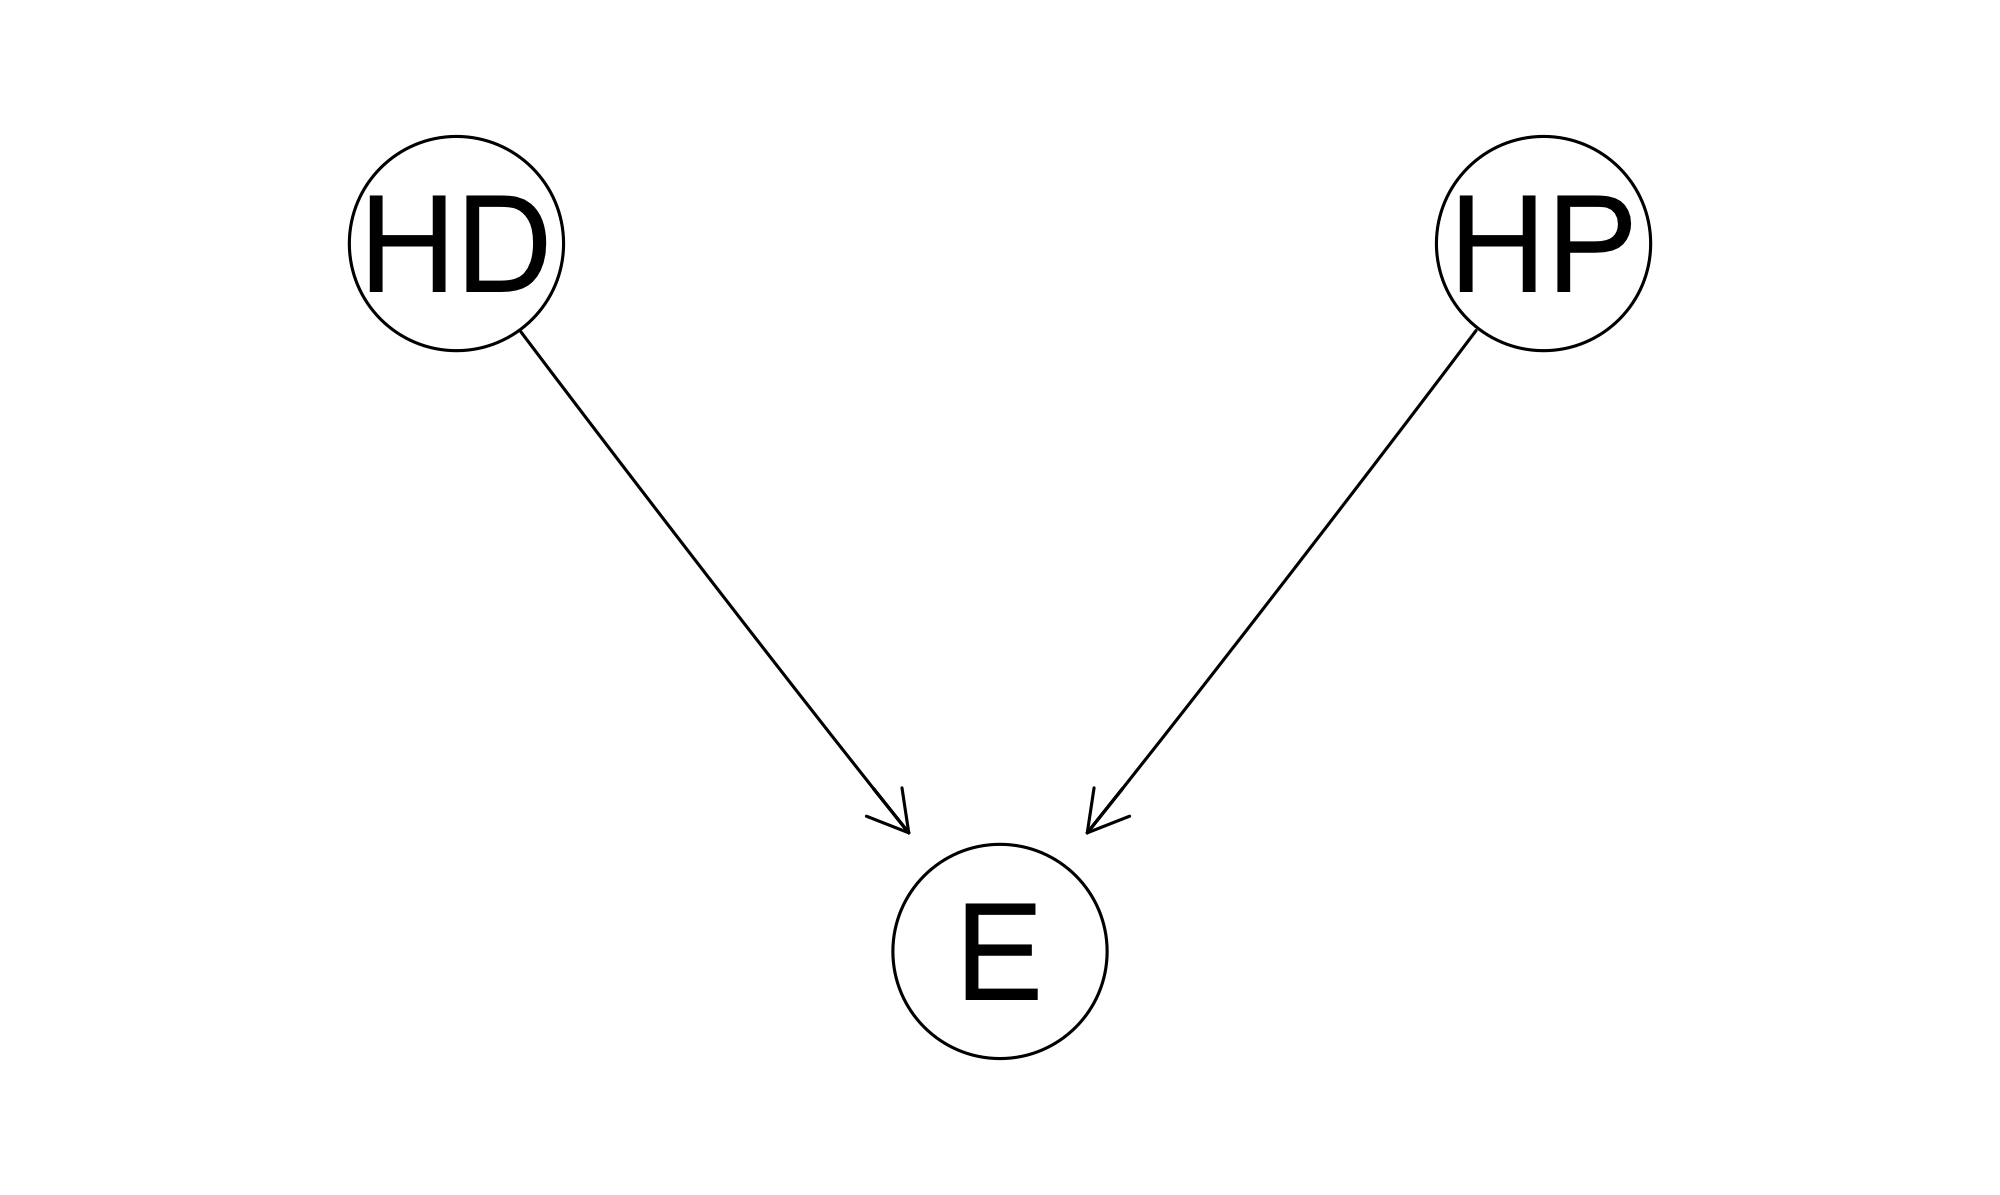
\includegraphics{STMdag.png}
\end{minipage} \hfill \begin{minipage}{0.4\textwidth}
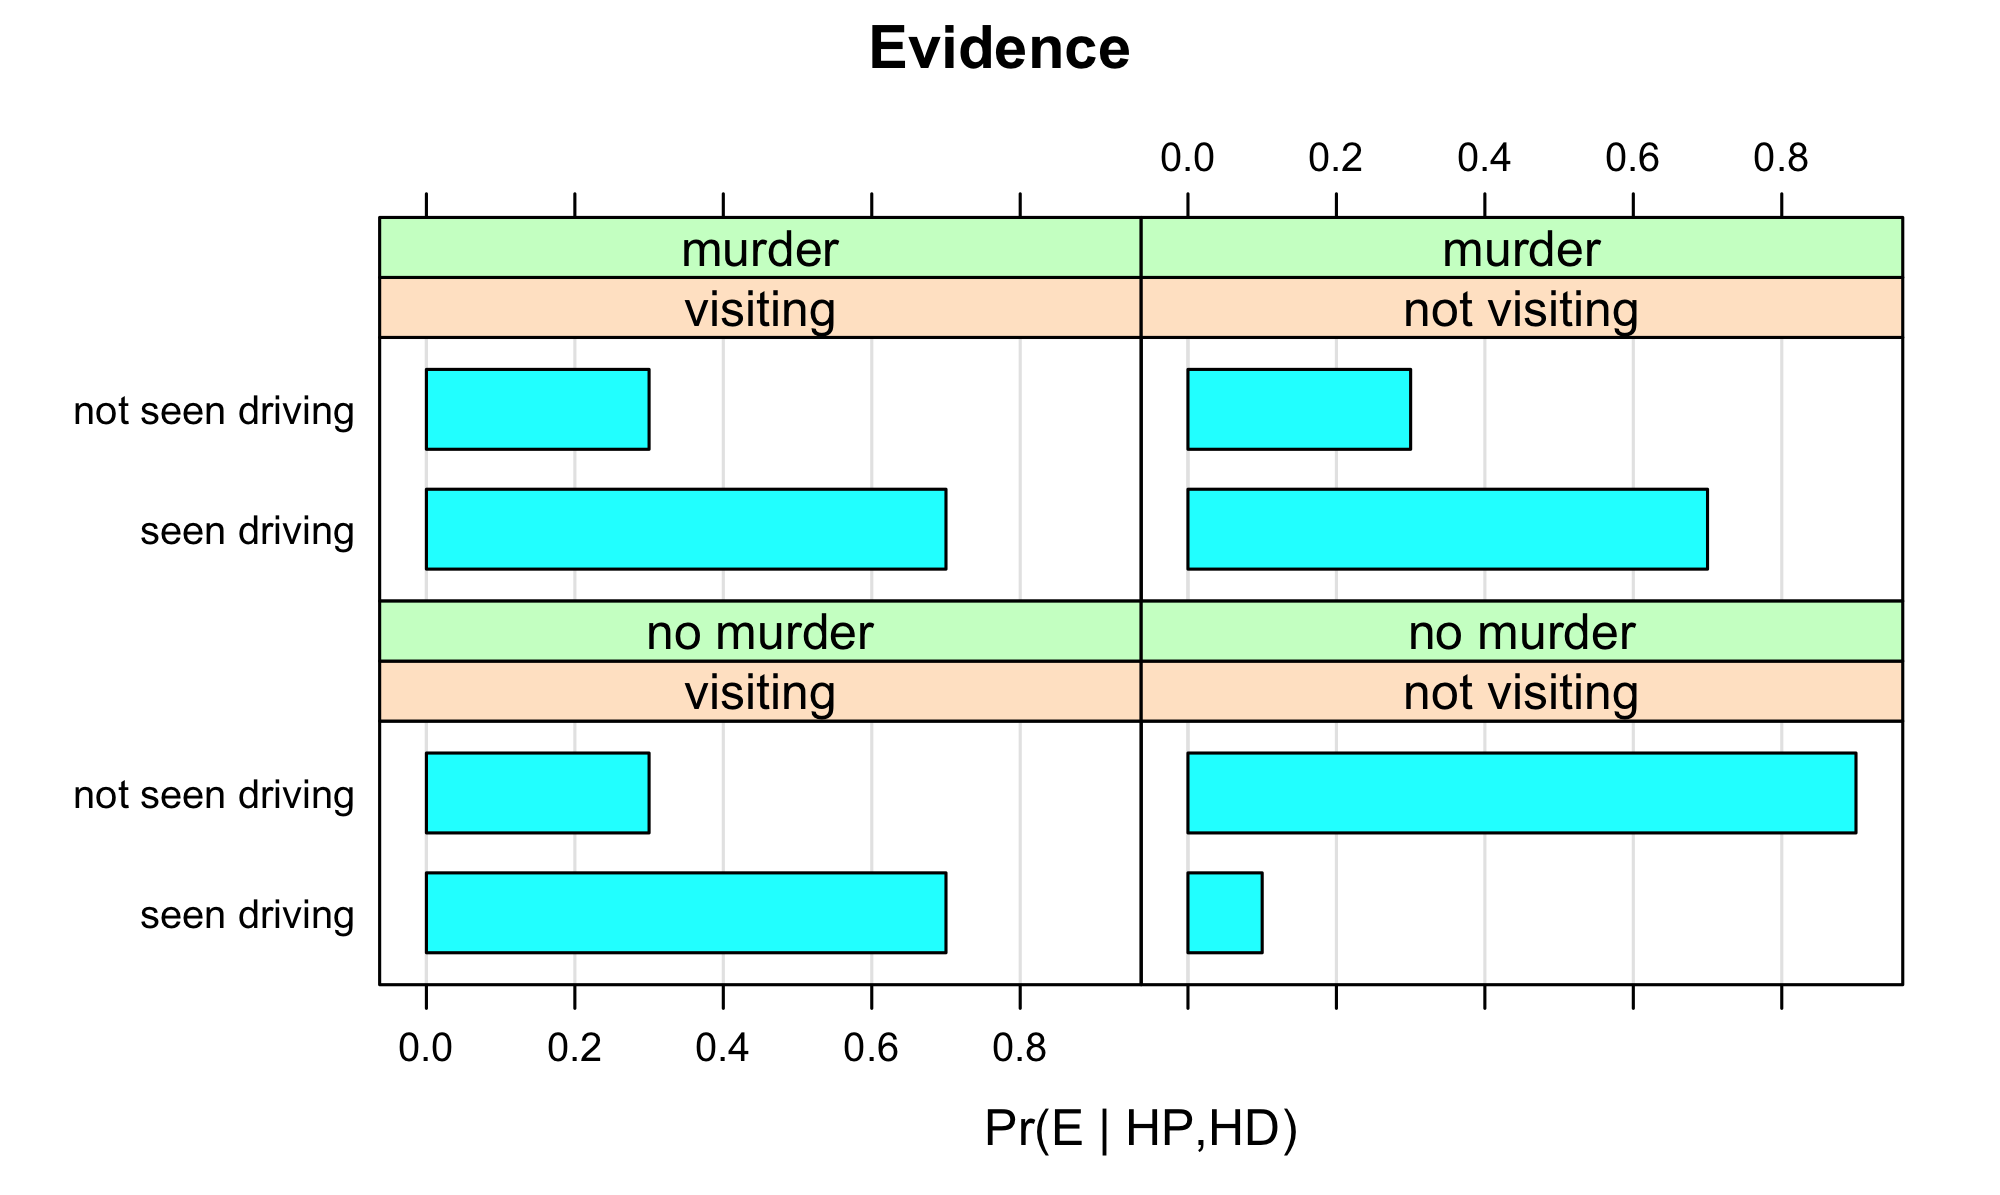
\includegraphics{STMpt.png}
\end{minipage}
\caption{Graphic model of Small Town Murder, with the  probability distribution of $E$.}
\label{fig:bayes_test4}
\end{figure}

\noindent
 Following the calculations in (de Zoete, Fenton, Noguchi, \& Lagnado,
2019), for exclusive and exhaustive hypotheses,
\(LR(E,H_d,\neg H_d)=1.75\), and similarly,
\(LR(E,H_p, \neg H_p)=1.75\), since \(P(E\vert H_d)=0.7\) and
\(P(E\vert \neg H_d)=0.4\). The likelihood ratio of the evidence, if it
is measured against exclusive and exhaustive hypotheses, is not equal to
one.\^{}(de Zoete et al., 2019 offer a slightly different solution to
the problem. They construct a Bayesian network with three hypotheses,
also exhaustive and exclusive: in town to visit mother, in town to
murder, out of town.) Such considerations should also generalize to
other paradoxes of relevance.

For instance, in the twins problem, the LR is 1 if the hypotheses are:
`the suspect committed the crime', and `the suspect's twin brother
committed the crime', but is not 1 f we consider the fairly natural
hypothesis that the defendant is innocent.

Similarly, in the food tray example, Bayesian network analysis shows
that the value of the evidence `prisoner withholds tray' for the
question who started the fight depends on a range of uncertain events
and other pieces of evidence (such as whether indeed a parcel he was
supposed to obtain was withheld; whether the prisoner inquired about
this; whether and how this inquiry was answered). Considered in this
context, the piece of evidence will not have a likelihood ratio of one
with respect to at least some choice of sensible hypotheses.

The general problem with the paradoxes of relevance is that in complex
situations there is no single likelihood ratio that corresponds to a
single piece of evidence. The problematic scenarios focus on a single
likelihood ratio based on non-exclusive or non-exhaustive hypotheses.
However, evidence can be relevant so long as it has a probabilistic
impact on a sub-hypothesis involved in the case, even without having a
recognizable probabilistic impact on the prosecutor's or defense's
ultimate hypotheses. When this happens, it is relevant, in agreement
with Rule 401 of the Federal Rules of Evidence. Bayesian networks help
to see how pieces of evidence can increase or decrease the probability
of different sub-hypotheses (de Zoete et al., 2019). Thus, while
likelihood ratios are useful, they need to be properly presented in the
context.

\section{\texorpdfstring{The cold-hit confusion
\label{sec:coldHitConfusion}}{The cold-hit confusion }}\label{the-cold-hit-confusion}

\todo{Added this intro here.} We have been quite negative in the last
two sections. What we are after, though, is a balanced perspective. We
are not saying that likelihood ratios should be disposed of: rather that
they should be reported for individual pieces of evidence and used to
evaluate the impact of combined evidence, but only when proper attention
is paid to the structure of the problem. To re-emphasize the utility of
likelihood ratios when care is paid to both the hypothesis formulation,
and to what the evidence in fact is, we illustrate it by showing how it
can be used to resolve a lengthy debate in legal evidence studies: the
value of a cold-hit DNA match.

DNA evidence is one of the most widely used forms of quantitative
evidence currently in use. It may be used to corroborate other evidence
in a case, or as the primary incriminating evidence. For example,
suppose different investigative leads point to an individual, Mark
Smith, as the perpetrator. The investigators also find several traces at
the crime scene left by the perpetrator. Laboratory analyses show that
the genetic profile associated with the traces matches Smith. In this
scenario, the DNA match corroborates the other evidence against Smith.
In contrast, suppose the police has no other investigative lead except
the traces left at the crime scene. Hoping to find the perpetrator, the
police run the genetic profile associated with the traces through a
database of profiles and find a match, a so-called \textbf{cold-hit}.
Cold-hit DNA matches have been the focus of intense discussion in recent
years. Since in cold-hit cases there is little or no other evidence,
cold-hit matches are often the primary item of evidence against the
defendant. Some believe that this circumstance weakens the case. Others
disagree. This debate illustrates how probability theory---in
particular, the likelihood ratio---can help to assess the strength of
evidence at trial. What follows examines some of the main arguments.

For concreteness, consider the California rape and murder case of Diana
Sylvester. In 2008, many years after the crime, John Puckett was
identified as a unique 9-loci match through a database search of 338,000
profiles. He was the only individual in the database who matched the
traces collected from the victim Diana Sylvester in 1972. According to
an expert witness, the particular pattern of alleles present in the
material was (conservatively) expected to occur randomly among Caucasian
men with a frequency of 1 in 1.1 million. This is the
\textbf{random match probability} (\textbf{RMP}). The random match
probability---often interpreted as the probability that someone who is
not the source would coincidentally match,
\(\pr{\textsf{match} \vert \neg \textsf{source}}\)---is a common measure
of the strength of a DNA match. The lower the RMP, the more strongly
incriminating the match. The rationale here is that a low random match
probability suggests that it is unlikely that two people would share the
same DNA profile. In line with what we already discussed, strictly
speaking, a match is a strong evidence that the defendant is the source
only if the probability that the person who left the traces (the
`source') would match is significantly greater than RMP. In practice,
when it comes to DNA evidence, it is often assumed that
\(\pr(\textsf{match} \vert \textsf{source})\) is very high.

Although clearly 1 in 1.1 million should not be confused with the
probability of Puckett's innocence (see \ref{sec:fallacies} for
details),\todo{check crossref later} the small figure indicates it is
very unlikely that a random person unrelated to the crime would match.
The match is therefore strong evidence of Puckett's guilt. Assuming that
the probability of a match if Puckett indeed was the source was
(practically) 1, the likelihood ratio is simply \(1.1 \times 10^6\).

During the pretrial hearing, however, Bicka Barlow, the DNA expert for
the defense, pointed out that this was a cold-hit case. No evidence tied
Puckett to the crime other than the cold-hit match, Puckett's previous
rape convictions, and the fact that he was in the area at the time of
the murder. In order to correctly assess the probative value of the
cold-hit match, Barlow argued, the random match probability should be
multiplied by the size of the database. The result of such a
multiplication is called the \textbf{database match probability}
(\textbf{DMP}). In Puckett's case, the multiplication of
\(\nicefrac{1}{1.1\times 10^6}\) by \(338,000\) resulted in a database
match probability of approximately .3.

\noindent which is a less impressive number than the original RMP (the
likelihood ratio for the DMP is approximately 3.25). According to this
calculation, it was no longer very unlikely that an unrelated person
from the database would match, and so the cold-hit DNA match was no
longer strong evidence of guilt. At least, this was Barlow's argument.

Barlow followed a 1996 report by the National Research Council called
NRC II (National Research Council, 1996), preceded by an earlier report
on DNA evidence called NRC I (National Research Council, 1992). NRC II
recommended precisely what Balrow did: that in cold-hit cases RMP should
be multiplied by the database size, yielding DMP. The underlying idea
was that the larger the size of the dataset, the higher the database
match probability, and the lower the strength of the match. This
correction was meant to guard against the heightened risk of mistaken
matches for the innocent people in the database. To see, however, if
this was sound advice, we need to look under the hood.

The NRC formed the Committee on DNA Technology in Forensic Science,
which issued its first report in 1992. In that report they advised
against using cold hit results as evidence, and insisted that only the
frequencies related to loci not used in the original identification
should be presented at trial, that is, that the evidence used to
identify the suspect should not be used as evidence against the suspect.

This recommendation has been criticized by many because it
underestimates the value of cold-hit matches. The problem was, given a
certain amount of evidence the expert, prior to suspect identification,
had to make a somewhat subjective decision of how to divide the evidence
into two items: one to be used only in the suspect identification, and
one to be used only in the trial itself as evidence against the suspect.
This overly limited the utility of the evidence and introduced an
unnecessary element of
subjectivity.\footnote{It also opened the gate for multiple testing with various evidence division points, and multiple testing leads to its own statistical problems. But let's put this issue aside.}

NRC II withdrew the earlier recommendation. However, the contrast
between low RMP and the frequency of DNA matches in actual database
searchers was indeed stark. For instance, the Arizona Department of
Public Safety searched for matching profiles in a database comprising
65,000 individuals. The search found 122 pairs of people whose DNA
partially matched at 9 out of 13 loci; 20 pairs people who matched at 10
loci; and one pair of people who matches at 12 loci. So it is not that
unlikely to find two people in a database who share the same genetic
profiles (examples of fairly high counts of DNA matches in database
searches was actually used by Barlow in the Diana Sylvester case). In
light of this contrast, NRC II recommended the use of DMP rather than
RMP. NRC II recommended also that in cold-hit cases the likelihood ratio
\(R\) associated with the DNA match should be divided by \(d+1\). Their
first recommendation was about a correction of the random match
probability, and this second recommendation is about the likelihood
ratio.

\todo{M: A lot of this is not about LR, so the reader now is confused and impatient since you promised you would talk abut the virtue of LR in DNA evidence evaluation. Need to say upfront this section is NOT about LR but about some other metrics, or else the reader would be lost. The next section is about LR, right?}

One argument by NRC employed an analogy involving coin tosses. If you
toss several different coins at once and all show heads on the first
attempt, this seems strong evidence that the coins are biased. If,
however, you repeat this experiment sufficiently many times, it is
almost certain that at some point all coins will land heads. This
outcome should not count as evidence that the coins are biased.
According to NRC II, repeating the coin toss experiment multiple times
is analogous to trying to find a match by searching through a database
of profiles. As the size of the database increases, so does the number
of attempts at finding a match, and it is more likely that someone in
the database who had nothing to do with the crime would match.

Another argument provided by NRC II compared a database trawl to
multiple hypothesis testing, and multiple hypothesis testing should be
avoided if possible in light of classical statistical methods.

Third, NRC II was concerned with the fact that in cold-hit cases the
identification of a particular defendant occurs after testing several
individuals. This concern has to do with the data-dependency of one's
hypothesis: seemingly, the hypothesis `at least one person in a given
database matches the DNA profile in question' changes its content with
the choice of the database.

We will start with the coin analogy. It is in fact unclear how the
analogy with coin tossing translates to cold-hit cases. Searching a
larger database no doubt increases the probability of finding a match at
some point, but is the increase as fast as the Arizona Department of
Public Safety examples and the coin analogy suggest? Quite crucially,
following (Donnelly \& Friedman, 1999) we need to pay attention to what
hypotheses are tested, what probabilistic methods the context
recommends, and what exactly the evidence we obtained is. For instance,
one hypothesis of interest is what we will call a
\emph{general match hypothesis}: \vspace{1mm}

\begin{tabular}{lp{8cm}}
(General match hypothesis) &
At least one of the profiles in the database of size $n$ 
matches the crime sample.
\end{tabular}

\vspace{1mm} \noindent The general match hypothesis is what NRC II seems
to have been concerned with. If for each data point RMP\(=\gamma\) were
held constant, and if random matches with different data points
\(\mathsf{match_1, match_2, \dots, match_d}\) excluded each other, the
probability of there being at least one random match would be the same
as the probability of their disjunction and could be calculated by the
additivity axiom:

\begin{align*}
\pr{\mathsf{at\,\,\, least\,\,\, one\,\,\, match}} & = \pr{\mathsf{match_1} \vee \mathsf{match_2} \vee \cdots \vee \mathsf{match_d}} \\
& = \sum_{i}^d \pr{\mathsf{match_i}} = \gamma \times d
\end{align*}

This calculation would result in the outcome recommended by NRC II, if
the value of the evidence were to be a function of the probability of
(General match hypothesis).

The first question is, whether a directly additive calculation should be
applied to database matches. Notice that in applications DMP does not
really behave like probability. Take a simple example. Suppose a given
profile frequency is \(.1\) and you search for this particular profile
in a database of size 10. Does the probability of a match equal
\(.1 \times 10=1\)? The answer is clearly negative. Multiplication by
database size would make sense if we thought of it as addition of
individual match probabilities, provided matches exclude each other and
so are not independent. Here is a coin analogy. Suppose I toss a die,
and my database contains \(n=\) three \emph{different} numbers: \(1, 2\)
and \(3\). Then, for each element of the database, the probability \(p\)
of each particular match is \(\nicefrac{1}{6}\), and the probability of
\emph{at least one} match is
\(\nicefrac{1}{6}+\nicefrac{1}{6}+\nicefrac{1}{6}=\nicefrac{1}{6}\times 3 = n\times p =\nicefrac{1}{2}\).
We could use addition in such a situation because each match excludes
the other matches, a condition that is not satisfied in the database
scenario.

Another reason why DMP is problematic can be seen by taking a limiting
case. Suppose everyone in the world is recorded in the database. In this
case, a unique cold-hit match would be extremely strong evidence of
guilt, since everybody except for one matching individual would be
excluded as a suspect. But if RMP were to be multiplied by the size of
the database, the probative value of the match as measured by DMP should
be extremely low. This is highly counter-intuitive.

Even without a world database, the NRC II proposal remains problematic,
since it sets up a way for the defendant to arbitrarily weaken the
weight of cold-hit DNA matches. It is enough to make more tests against
more profiles in more databases. Even if all the additional profiles are
excluded (intuitively, pointing even more clearly to the defendant as
the perpetrator), the NRC II recommendation would require to devalue the
cold-hit match even further. This, again, is highly counter-intuitive.

Perhaps a somewhat more sensible answer is obtained by assuming the
independence of \(\mathsf{no match}\) for the members of the database
and deploying a solution similar to the one used in the birthday
problem. Here, the idea would be---assuming matches for different data
points are independent and have constant RMP --- to calculate:

\begin{align*}
\pr{\mathsf{match}} & = 1 - \pr{\mathsf{no match}}\\
& = 1 - (1-\gamma)^d
\end{align*}

\noindent where \(\gamma\) is RMP, and \(d\) is the database size. This
would be in line with using the binomial distribution to calculate the
probability of no match:

\begin{align*}
\mathsf{dbinom}(0,d,\gamma) & = {n \choose 0} \gamma^0 (1-\gamma)^{d-0}\\
& = 1 \times 1 \times (1-\gamma)^d
\end{align*}

Now, assuming indeed that \(\gamma\) is constant and that matches
between data points are independent, the dependence of the probability
of at least one match on the database size can be pictured as in Figure
\ref{fig:puckett}.

If we use the RMP and database size used in the Puckett case, the
calculated probability of at least one match is 0.2645501. Not exactly
the DMP postulated by the defendant, but pretty close. The question is,
should this number be the probability used to evaluate the evidential
impact of the cold hit?

One problem is, whether the independence assumption is satisfied in the
database search problem is unclear. After all, if you are informed about
the match frequencies in the database, and they teach you that since two
arbitrary database points quite likely do not match, if the sample
matches one of them, it is less likely to match the other one. And the
independence assumption is not benign. We will illustrate it with a
somewhat distand, but a very striking example, coming from (Barnett,
2020). Suppose you consider whether your effort of casting a vote in the
upcoming election is worth it in a context where there are 500k other
voters. One of the probabilities you might be interested in is the
probability that your vote would make a difference. If we apply the
binomial model to the problem, the probability that a candidate will
receive exactly \(k\) votes if \(n\) people vote is supposed to be
\({n \choose k} p^{k} (1-p)^{(n-k)}\), where votes of the population
members are supposed to be independent and estimated to have the same
probability \(p\) of being for the candidate. For instance, if 500k
people vote and \(p= 0.5\), the probability that the candidate will
receive exactly 250k votes is 0.0011284, which is around
\nicefrac{1}{886} and much higher than \(\nicefrac{1}{n}\). This fairly
high chance made some claim that the chance that your voice is decisive
if the chances are equal is fairly high in such circumstances. However,
note that if \(p=.505\), the probability that the candidate will receive
exactly 250k votes is \ensuremath{1.5651281\times 10^{-14}}, which is
less than one in a trillion. This lead some (Brennan, 2012;
\emph{Democracy and decision}, 1993) to claim that outside of the very
specific circumstances, decision-theoretic arguments for the rationality
of voting are hopeless. Barnett, however, points out that such a
sensitivty to success probability simply makes the binomial model
inappropriate for the voting context, observing that its calculations
also disagree with empirical estimates which are not too far from
\(1/n\) (Gelman, Katz, \& Tuerlinckx, 2002; Gelman, King, \& Boscardin,
1998; Mulligan \& Hunter, 2003). This sensitivity arises, because within
the binomial model the more trials (voters) there are, the more tightly
the results will tend to cluster around the probablity of success. To
observe how unrealistic that is, keep \(p=.505\) and ask yourself how
probable it is that the voting result will be between \(50.4\%\) and
\(50.6\%\). Sure, this outcome might be quite likely, but the binomial
certainly overstimates it at 0.8427212. Another unrealistic estimate
obtained by the binomial model is the estimate of the probability of an
upset (that the leading candidate will lose). With \(p=.505\) this is
\(\mathsf{pbinom(249999,500000,.505)}\), which turns out to be extremely
and unrealistically low: \ensuremath{7.5994495\times 10^{-13}}.

\todo{M: Pretty interesting, but in the voting model, it seems that feedback mechanisms betewen voters affect behaviour, but not so in the genetic case. Can you spell out the analogy more clearly?}

\begin{figure}[h]

\begin{center}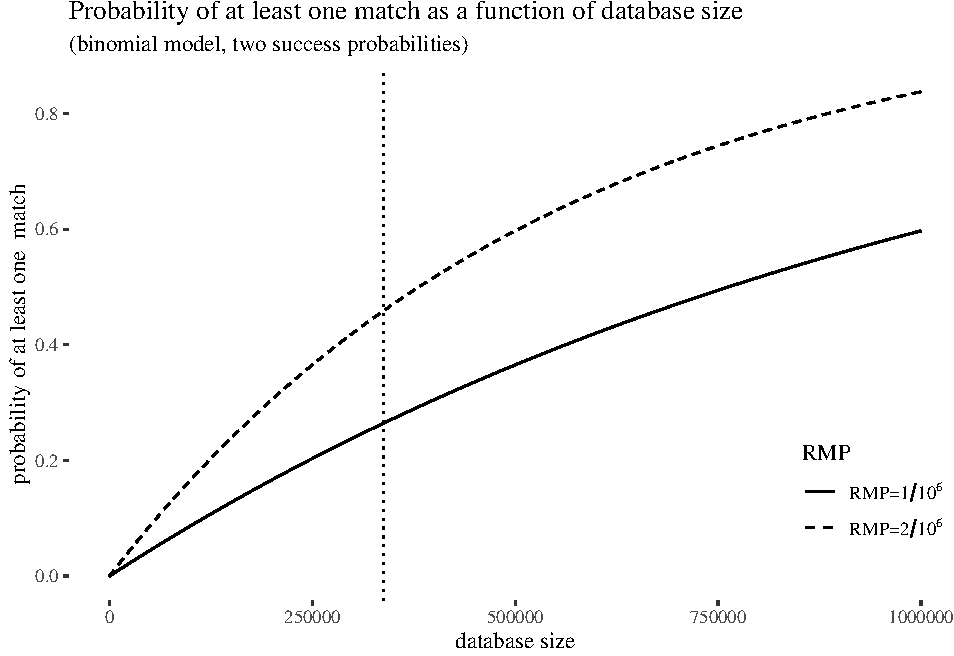
\includegraphics[width=0.8\linewidth]{lr-chapter3_files/figure-latex/fig-puckett-1} \end{center}
\label{fig:puckett}
\caption{Binomial model of the database search problem. The probability of at least one match depending on the database size, assuming independence and constant RMP used in  the Puckett case as compared with the binomial estimate for p=2/1.1e6 (dashed line). The actual database size marked with a vertical line."}
\end{figure}

Coming back to our original problem, the binomial estimate of the
probability of a match is also quite sensitive to RMP, as illustrated in
Figure \ref{fig:puckett}. The bottom line is that if we have reasons to
think the independence assumption is not satisfied, the binomial model
is not appropriate. So, it seems, it is not appropriate for the database
match problem either.

The binomial model, however, is useful, in its simplicity, for
illustrating an important distinction whose conflation underlies one of
the involved arguments. You might have been surprised learning that
while the expert testified that RMP on 9 loci for Puckett was 1 in 1.1
million, the Arizona Department of Public Safety found 122 9-loci
matches among 65,000 individuals. After all, 122/65000 is 0.0018769,
which is much higher than the reported RMP.

Crucially, notice that there is a difference between having a sample and
looking for a match in a database of size \(n\) and taking a database of
size \(n\) and checking all pairs that occur within it for a match. In
the former case, you are making \(n\) comparisons. In the latter case,
the number of comparisons is \({n \choose 2}\), which is much higher. If
\(n=65000\), there are \ensuremath{2.1124675\times 10^{9}} pairs to
compare, so while the binomial estimate of the probability of at least
one match for \(n\) comparisons (the former case) is 0.057379, it is
approximately 1 for \({n \choose 2}\) comparisons. For the impact it has
on the Arizona Department of Public Safety statistics, consider the
binomial estimate of the probability of at least 122 matches among all
pairs as a function of the database size, even for relatively low
database size range (up to 50000), as illustrated in Figure
\ref{fig:Arizona}.

\begin{figure}[h]

\begin{center}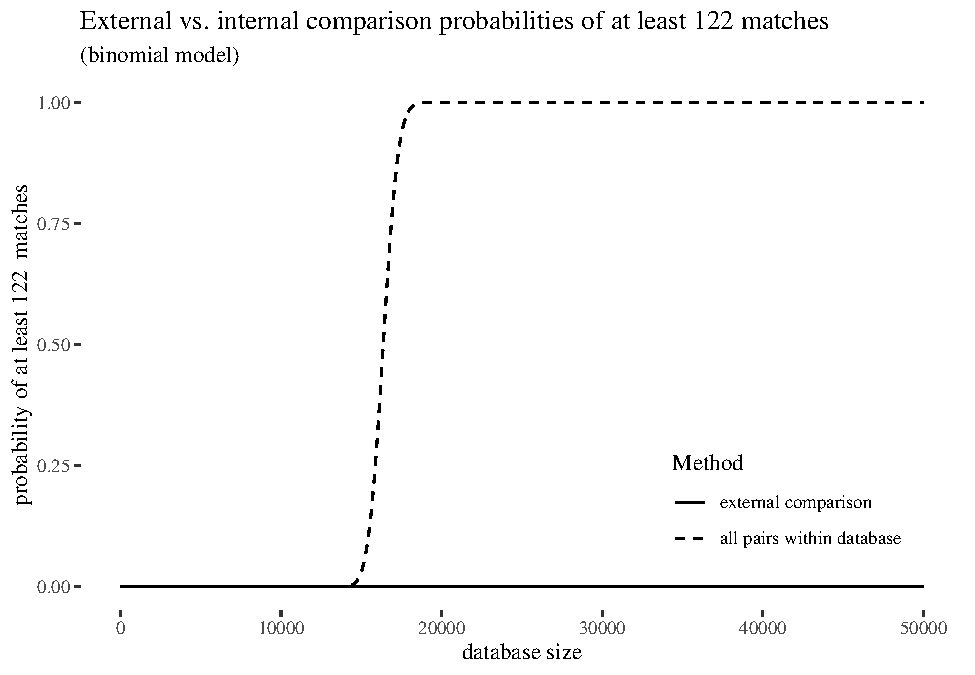
\includegraphics[width=1\linewidth]{lr-chapter3_files/figure-latex/fig-Arizona-1} \end{center}
\caption{Binomial model of the database search problem. The probability of at least 122 matches depending on the database size for n comparisons with an external sample, and for all possible pairs among n datapoints (dashed), assuming RMP=1/1.1e6.}
\label{fig:Arizona}
\end{figure}

From this perspective, it is no surprise there were so many matching
pairs among all the pairs from the database. Unfortunatelly, this
frequency does not estimate the probability of at least one match in the
set-up we are actually interested in. After all, in a cold-hit senario
we do have a sample outside of the database and make \(n\) comparisons,
instead of testing all possible pairs from the database for a match.

\todo{M: In general this section needs more signposting for guiding the reader. This last arguemnt seems to be an add-on.}

Before we move on, note how the Arizona statistics constitute some
empirical evidence against the adequacy of the binomial model. While the
binomial estimate probability of at least 122 matches with an external
sample for \(n=6500\) is pretty much 0, let us look at the most likely
number of matches if we test \({6500 \choose 2}\) pairs, as estimated by
the binomial model. We illustrate it with an 89\% highest density
inverval in Figure \ref{fig:ArizonaDensity}. So, if the expert's
estimate and the binomial model are both adequate, we indeed should be
surprised by the presence of 122 matches. But this is because this
number is suprisingly low: instead we should expect a much higher
number, around 2000 of them! OF course, it is unlikely that in fact all
possible pairs have been compared, and it is hard to evaluate this
evidence against the binomial model unless we know the exact number of
comparisons made.

\begin{figure}[h]

\begin{center}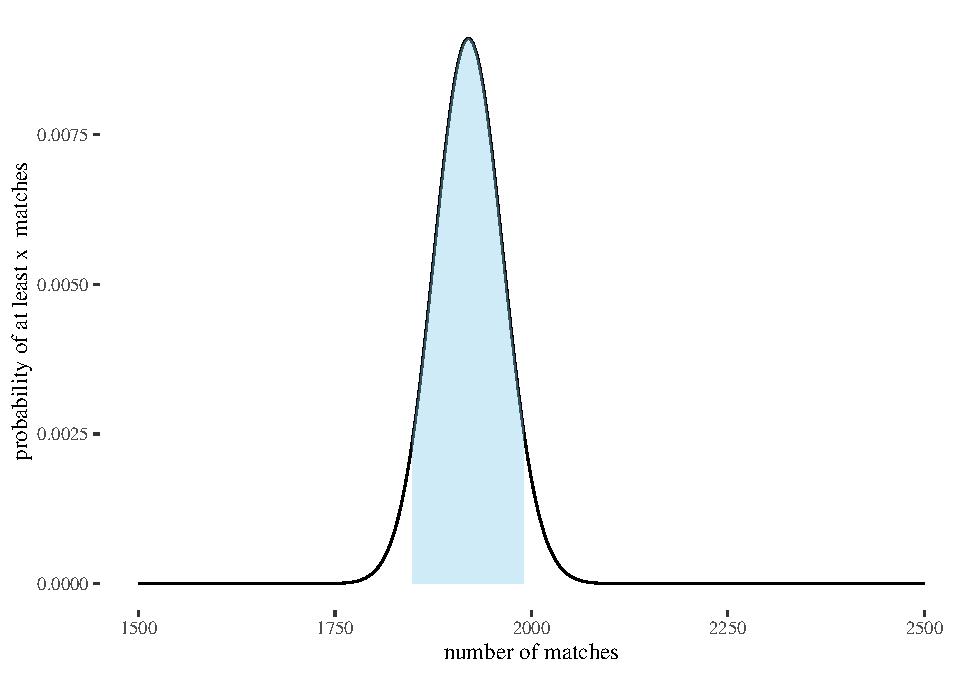
\includegraphics[width=1\linewidth]{lr-chapter3_files/figure-latex/fig:ArizonaDensity-1} \end{center}
\caption{Binomial probability density of  n matches in pairwise comparison within a database of size 65000, assuming $p=1/1.1e6$, with 89\% highest density interval $=(1849,1990)$ shaded in blue.}
\label{fig:ArizonaDensity}
\end{figure}

Now that we used the imperfect binomial model to clear up at least one
confusion, let us put it aside, and focus on an even deeper problem with
using the probability of (General match hypothesis) instead of RMP in
evidence evaluation. Probabilistic epistemology recommends that once we
obtain new evidence, our new degrees of belief should be the
probabilities obtained by conditionalizing on this evidence. Crucially,
we should update on the total evidence we obtained rather than only on a
part of it. Here the question is, does (General match hypothesis)
exhaust what we have learned from our database match?

To get us started thinking about this question, consider a coin analogy
which Donnelly \& Friedman (1999, p. 950) found more adequate than the
one proposed by the NRC. Imagine a biased coin whose physical appearance
is indistinguishable from the fair coins in a piggy bank. The biased
coin is the perpetrator and the piggy bank is the database containing
innocent people. After the biased coin is thrown into the bank with the
other coins, someone picks out a handful of coins at random and flips
each of them twenty times. Each coin lands heads approximately ten
times---except for one coin, which lands heads on all twenty flips. The
fact that other coins seem unbiased makes the claim that this one is
biased\\
better supported.

Coming back to DNA matches, think about the following scenario: first,
you identified the suspect by some means other than a database trawl.
Then, it turned out his DNA profile matches the crime scene stain. Fine,
here it seems uncontroversial that this constitutes strong further
incriminating evidence. Now, imagine a further database search in a
database not containing this suspect finds no matches. Would you think
that this information supports the guilt hypothesis? If your answer is
yes, then you do have the intuition that the lack of matches with other
people (whose profiles, in this particular case, happen to be in a
database) strengthens the evidence.

The key lesson here (and in the complete-world database scenario we
already discussed) is that we not only learned that there was a match in
the database of size \(n\), but also that in \(n-1\) cases there was no
match, and this information also has evidential value. In line with
this, contrary to NRC II, Donnelly \& Friedman (1999) argues that if
potential suspects in the database are excluded as sources, this should
increase, not decrease, the probability that the defendant who matches
the crime traces is the source. A cold-hit match, then, is stronger and
not weaker evidence of guilty than ordinary DNA matches.

Before moving on to a better model that captures how this could be, let
us look at another argument put forward by NRC, an analogy to multiple
hypothesis testing. NRC claimed that there is an analogy between
searching for a match in a database and multiple hypothesis testing,
which is a dubious research practice. In classical hypothesis testing,
if the probability of type I error in a single test of a hypothesis is
5\%, the probability of at least one type I error will increase by
testing the same hypothesis multiple times. In analogy---the argument
goes--- we need to correct for the increased risk of type I error, and
just as the Bonferroni correction requires that the \(p\)-value
threshold be divided by the number of tests, NRC II requires that the
estimated probability of a random match should be multiplied by the
number of comparisons.

This analogy with multiple testing, however, is misplaced. As Balding
(2002) points out, multiple testing consists in testing the
\textit{same} hypothesis multiple times against new evidence. In
cold-hit cases, no such multiple testing is involved. Rather, multiple
hypotheses---each concerning a different individual in the
database---are tested only once and then excluded if the test is
negative. From this perspective, for each \(1 < i <n\), the following
hypothesis is tested: \vspace{1mm}

\begin{tabular}{lp{8cm}}
(Particular match hypothesis) &
Profile $i$ in the database matches the crime sample.
\end{tabular}

\vspace{1mm} \noindent and the hypothesis that the defendant is the
source was one of the many hypotheses subject to testing. The cold-hit
match supports that hypothesis and rules out multiple other hypotheses.

\section{\texorpdfstring{Likelihood ratio and cold-hit DNA matches
\label{sec:cold-hit}}{Likelihood ratio and cold-hit DNA matches }}\label{likelihood-ratio-and-cold-hit-dna-matches}

To find a better parth towards the resolution of the database search
problem, let us look at another recommendation of NRC II, that in
cold-hit cases the likelihood ratio \(R\) associated with the DNA match
should be divided by \(n+1\), where \(n\) is the database size. This
approach has been defended defended by (Stockmarr, 1999), who points out
that since the suspect is identified after the databases search, the
hypothesis is formulated \textit{ad hoc}. Without the correction, then,
the likelihood ratio would be data-dependent. For instance, he insists
that hypotheses such as \emph{JS was one of the crime scene donors} are
evidence-dependent in the case of database search, ``since we had no way
of knowing prior to the search that Smith would be the person that
matched'' (p.~672). Instead, Stockmarr claims, we should evaluate LR
using hypotheses that can be formulated prior to the search, such as
\emph{the true perpetrator is among the suspects identified from the database}.
And indeed, the likelihood of this hypothesis is as NRC II suggests,
\(\nicefrac{k}{np}\), where \(k\) is the number of matching profiles,
\(n\) the database size, and \(p\) the random match probability (see
Stockmarr, 1999 for a derivation).

Dawid, in a discussion with Stockmarr (Dawid \& Stockmarr, 2001) points
out that Stockmarr's hypotheses, while not depending on the result of
the search, depend on the data themselves (because they change with the
database size). More importantly, he also indicates that Stockmarr's
hypotheses are composite and the assessment of LR therefore requires
additional assumptions about the priors. Once these are used with
Stocmarr's own LR, the posterior is the same as the one obtained using
the methods proposed by the critics of NCR II. This is a particular case
of a general phenomenon that we will discuss later on: different
hypotheses might result in different LR, but be equivalent conditional
on the evidence, and so result in the same posterior probabilities. This
general phenomenon indicates how LR on its own might be insufficiently
informative.\footnote{See however, Stockmarr's own reply
  (\emph{ibidem}).}

Putting Stockmarr's defense and its problems aside, the NRC II
recommendation is questionable on more principled grounds. Suppose \(R\)
is not too high, say because the identified profile is common since the
crime scene DNA is degraded and only a few markers could be used. Then,
\(n+1\) can be greater than \(R\), so \(R/(n+1)<1\). The match would
then be exculpatory, a very counter-intuitive result. Moreover, if the
defendant on trial is the source, the probability that he would match is
practically 1. If he is not, the probability that he would still match
equals the random match probability. Neither of these probabilities
change because other suspects have been tested in the database search.
In fact, if potential suspects are excluded as potential sources, this
should increase, not decrease, the probability that the defendant who
matches the crime traces is the source.

A more principled way to assess cold-hit matches based on the likelihood
ratio, exists. The proposal draws from the literature on the so-called
\textbf{island problem}, studied by (Dawid, 1994; Dawid \& Mortera,
1996; Eggleston, 1978). Let the prosecutor's hypothesis \(H_p\) be `The
suspect is the source of the crime traces' and the defense's hypothesis
\(H_d\) be `The suspect is not the source of the crime traces'. Let
\(E\) be the DNA match between the crime stain and the suspect (included
in the database) and \(D\) the information that none of the \(n-1\)
profiles in the database matches the crime stain. The likelihood ratio
associated with \(E\) and \(D\) should be (Balding \& Donnelly, 1996;
Taroni et al., 2014):

\begin{align*}
V & = \frac{\pr{E,D\vert H_p}}{\pr{E,D\vert H_d}}.
\end{align*}

Since \(\pr{A\wedge B}=\pr{A\vert B}\pr{B}\), for any statement \(A\)
and \(B\), this ratio can be rewritten as:

\begin{align}\label{eq:lrdna1}
V & = \frac{\pr{E\vert H_p,D}}{\pr{E\vert H_d,D}} \times \frac{\pr{D\vert H_p}}{\pr{D\vert H_d}}.
\end{align}

\noindent The first ratio in \eqref{eq:lrdna1} is roughly
\(\nicefrac{1}{\gamma}\), where \(\gamma\) is the random match
probability. The second ratio--- call it the
\textbf{database search ratio}---requires some more work. Consider first
the denominator \(\pr{D \vert H_d}\). If the suspect is not the source
(\(H_d\)), someone else is, either someone who is in the database or
someone not in the database. Let \(S\) stand for
\textsf{The  source is someone in the database.} By the law of total
probability,

\begin{align}\label{eq:dnaLOTP}
\pr{D\vert H_d} & = \pr{D\vert S, H_d} \pr{S\vert H_d} + \pr{D\vert \neg S, H_d} \pr{\neg S \vert H_d}. 
\end{align}

If the source is someone in the database (\(S\)) and the suspect is not
the source (\(H_d\)), it is very unlikely that no one in the database
would match (\(D\)), so \(\pr{D\vert S, H_d}\approx 0\). The equality in
\eqref{eq:dnaLOTP} therefore simplifies to: \vspace{-4mm}

\begin{align*}
\pr{D\vert H_d} & =  \pr{D\vert \neg S, H_d} \pr{\neg S \vert H_d}, 
\end{align*}

\noindent The database search ratio would therefore be:

\begin{align*}
\frac{\pr{D\vert H_p}}{\pr{D\vert H_d}} & = \frac{\pr{D\vert H_p}}{\pr{D\vert \neg S, H_d} \pr{\neg S \vert H_d}}.
\end{align*}

\noindent Note that \(\pr{D\vert H_p}=\pr{D\vert \neg S, H_d}\) because
whether the suspect is the source (\(H_p\)) or not (\(H_d\)) does not
affect whether there is a match in a database that does not contain the
source (\(\neg S\)). Let the probability that no person in the database
other than the suspect would match (\(D\)), assuming the suspect was in
fact the source, be \(\psi_{n-1}\). Notice that
\(\pr{D\vert \neg S, H_d}\) is the probability that no one other than
the suspect matches in the database that does not contain the real
source, if the suspect is not the source. So this conditional
probability can also be estimated as
\(\psi_{n-1}\).\footnote{If the prior probability that the perpetrator is in the database was high, the calculations would need to be different. But normally, this prior is not too high.}
Let \(\pr{S | H_d}=\varphi\). The database search ratio then would
reduce to \vspace{-2mm}

\begin{align*}
\frac{\pr{D\vert H_p}}{\pr{D\vert H_d}} & = \frac{1}{1-\varphi}.
\end{align*}

\noindent As the database gets larger, \(\varphi\) increases and the
database search ratio also increases. This ratio equals one only if no
one in the database could be the source, that is, \(\varphi=0\).\\
Since the likelihood ratio \(V\) of the cold-hit match results by
multiplying the likelihood ratio of the DNA match and the database
search ratio, \(V\) will always be greater than the mere likelihood
ratio of the match (except for the unrealistic case in which
\(\varphi=0\)) . Thus, a cold-hit DNA match should count as stronger
evidence than a DNA match of a previously identified suspect.

Dawid \& Mortera (1996) study different database search strategies and
consider the possibility that information about the match is itself
uncertain, but the general point remains. Under reasonable assumptions,
ignoring the database search would give a conservative assessment of the
evidentiary strength of the cold-hit match. Donnelly \& Friedman (1999),
with slightly different assumptions, derived the formula
\(R \times [1+md/N]\), where \(R = 1/\gamma\), \(d\) is the database
size, \(N\) the number of people in population not in database, and
\(m\) is an optional multiplier reflecting how much more likely persons
in the database are though to be the source when compared to the rest of
the population. The expression cannot be less than \(\gamma\). If no
other profile has been tested, \(d=0\) and LR is simply the regular DNA
match LR. If \(N\) is zero, that is, everyone in population is in the
database, the result is infinitely large.

This proposal is able to accommodate different apparently competing
intuitions. First, consider the intuition that as the size of the
database grows, it is more likely that someone in the database would
match. This intuition is captured by the fact that \(\varphi\) increases
proportionally to the size of the database even though this increase
does not imply that the evidential value of the cold-hit match should
decrease. Second, there is intuitive resistance to basing a conviction
on a cold-hit match, although this resistance is less strong in case of
an ordinary match (more on this later in Section
\ref{sec:naked}).\todo{Fix crossref later} This preference for
convictions based on an ordinary DNA match seems in tension with the
claim that a cold-hit match is stronger evidence of guilt than an
ordinary match. There is a way to make sense of this, though. The key is
to keep in mind that the evidentiary strength---measured by the
likelihood ratio---should not be confused with the posterior probability
of guilt given the evidence. Even if a cold-hit match is stronger
evidence of guilty, this fact does not imply that the posterior
probability of the defendant's guilt should be higher.\\
If the cold-hit match is the only evidence of guilt, the posterior
probability of guilt may well be lower compared to cases in which other
evidence, such as investigative leads, supplements the DNA match. This
lower posterior probability would justify the intuitive resistance
towards convictions in\\
cold-hit cases, despite the fact that a cold-hit match alone is stronger
evidence than a dna match obtained otherwise and taken on its own.
Moreover, it is possible that the intuitive assesment of cold-hit
evidence takes to some extent the impact of false positive probability
into account.

\todo{M: We need a proper conclusion here. Now it feels as thought LR are a good thing, at leats for cold-hits. But is this just an exception? Do LR have a very narrow applicability, say only for DNA evidence? So where do we stand exactly? And what about BF and Bayesian networks and priors? Need general morals here.}

\todo{I think I now reiterated our point too many times throughought the chapter, we'll discuss this.}

\section{\texorpdfstring{Confirmation measures
\label{sec:confirmation}}{Confirmation measures }}\label{confirmation-measures}

At this point a philosophically minded reader might recall that there is
an important notion in the vincinity---that of confirmation---and that
there is a vast philosophical literature on probabilistic explication of
that notion. Natural questions arise: how is the notion of confirmation
related to the notion of evidence strength, and why almost none of the
probabilistic explications of confirmation have not been deployed in
legal probabilism?

The key question behind the enterprise we are going to take a look at
is: when does a piece of evidence confirm a theory, and how are these
requirements to be explicated probabilistically to agree with both
successful scientific practice and sensible philosophical principles?
The hope is that having answered these questions would facilitate both
rational reconstructions of various developments in the history of
science, and a critical evaluation of various ongoing scientific
investigations.

The underlying probabilistic idea is that the level of confirmation of a
theory (\(T\)) by a piece of evidence (\(E\)) is a function of an
agent's degrees of belief. The first stab might be, let's simply
identify the confirmation level with \(\pr{T \vert E}\). This, however,
is way too quick. Multiple factors come into the assessment of this
conditional probability, and two agents can agree on the extent to which
\(E\) confirms \(T\) without agreeing on the posterior probability of
\(T\) (identified with \(\pr{T \vert E}\)), because the agents might
disagree about the prior probability of \(T\) and this might have an
impact on the posterior.

Still, some requirements on confirmation measures can be formulated in
terms of probabilities. One usual assumption (Sprenger \& Hartmann,
2019) is that the level of confirmation is to be a continuous function
of \(\pr{T}\) and \(\pr{E\vert T}\) which is non-decreasing in the first
argument and non-increasing in the second argument. That is, increasing
the prior, should not lower the confirmation level, and increasing the
likelihood should not increase the confirmation level. Let's call this
condition the \emph{prior-posterior dependence}.\footnote{Some
  formulations (Crupi, 2015) are a bit more general and include
  background knowledge \(K\). In that setting, the corresponding
  requirement is called \emph{Formality} and takes the confirmation to
  be a function of \(\pr{H \et E \vert K}, \pr{H\vert K}\) and
  \(\pr{E\vert K}\). For the sake of simplicity, we will suppress the
  reference to \(K\), unless required by the context.}

One consequence of the prior-posterior-dependence---called
\emph{Final Probability Incrementality} is that confirmation of \(T\) by
\(E\), \(c(T,E)\) should track the posterior order-wise, that is
\(c(T,E)>c(T,E')\) just in case \(\pr{T\vert E} > \pr{T\vert E'}\).

Another requirement is that there should be a neutral point \(n\) such
that \(E\) confirms (disconfirms) \(T\) just in case \(c(T,E)>n\)
(\(c(T,E)<n\)) and is neutral exactly at \(n\). This is called the
\emph{qualitative-quantitative bridge}.

Yet another requirement is \emph{local equivalence}. Theories that are
logically equivalent given the evidence should receive equal
confirmation from this evidence. Interestingly, all confirmation
measures which satisfy prior-posterior dependence,
qualitative-quantitative bridge, and local equivalence are strictly
increasing functions of \(\pr{H \vert E}\). Such measures are said to
explicate confirmation as \emph{firmness of belief}. Moreover, all
functions satisfiying these three conditions are ordinally
equivalent.\footnote{Measure $c$ is ordinally equivalent to measure $c'$ just in case always $c(E , T) \gtreqqless c(E', T')$ iff $c'(E , T) \gtreqqless c'(E' , T')$.}

However, another notion of confirmation seems often at play. For
instance, even if the posterior \(T\) is low, one might still think that
a given experiment still speaks strongly in favor of \(T\). And
relatedly, \(E\) can lower the posterior of \(T\) while still leading
the posterior to be sufficiently high for the firmness confirmation
measure to be above the neutrality threshold. Another feature of
confirmation as firmness is that if, in this sense, \(T\) confirms
\(H\), then for any \(H'\) that is excluded by \(H\), \(T\) disconfirms
\(H'\). But now think of the small town murder scenario discussed in
Section XXXX\todo{ref}: the fact that the suspect was seen in town seems
to support both the prosecution hypothesis that he committed the murder,
and the defense hypothesis, that he was in town to visit his mother.
Confirmation as firmness cannot capture such intuitions, as relevance
cannot be captured as a function of the posterior alone.

For such reasons, following the second edition of (Carnap, 1962), it is
customary to distinguish another notion in the vincinity: confirmation
as increase in firmness of belief. If we replace local equivalence with
tautological equivalence \(c(T, \top) = c(T', \top)\), where \(\top\) is
a logical tautology---the idea being that hypotheses are equally
supported by empty evidence---we end up with another class of
confirmation measures, those meant to capture
\emph{probabilistic relevance}. On this approach, \(E\) confirms
(disconfirms) \(T\) just in case \(\pr{H \vert E} > \pr{H}\)
(\(\pr{H \vert E} < \pr{H}\)).

Here is a list of key confirmation measures available on the market
(Sprenger \& Hartmann, 2019), normalized so that they all have neutral
points at 0:

\begin{align}
\tag{Difference}  D(T,E) & = \pr{T\vert E} - \pr{T}\\
\tag{Log-ratio}  Lr(T,E) &  = log\left(\frac{\pr{T\vert E}}{\pr{T}} \right) \\
\tag{Log-likelihood}   LL(T,E) & = log\left(\frac{\pr{E \vert T}}{\pr{E \vert \n T}} \right)\\
\tag{Kemeny-Oppenheim}  K(T,E) & = \frac{\pr{E\vert T} - \pr{E \vert \n T}}{\pr{E \vert T} + \pr{E \vert \n T}} \\
\tag{Generalized entailment}  Z(T,E) & = \begin{cases}
\frac{\pr{T\vert E - \pr{T}}}{1-\pr{T}} & \mbox{ if } \pr{T \vert E} \geq \pr{T}\\
\frac{\pr{T\vert E - \pr{T}}}{\pr{T}} & \mbox{ if } \pr{T \vert E} < \pr{T}
\end{cases} \\
\tag{Christensen-Joyce} S(T,E) & = \pr{T \vert E} - \pr{T \vert \n E} \\
\tag{Carnap}  C(T,E) & = \pr{E}(\pr{T\vert E} - \pr{T})\\
\tag{Rips} R(T\vert E) & = 1 - \frac{\pr{\n T\vert E}}{\pr{-T}}
\end{align}

(Log-likelihood), our good old likelihood ratio, and (Kemeny--Oppenheim)
are ordinally equivalent (and no other pair on the list is). Further
grouping and assessment of the confirmation measures for a given purpose
is facilitated by the following facts:

\begin{itemize}
\item
  One might require that \(E\) always confirms the disjunction of
  excluding hypotheses more than one of them just in case it also
  confirms the other one (\emph{disjunction of alternative hypotheses}).
  This can happen only if the confirmation measure is a strictly
  increasing function of the difference measure. Whether this is an
  intuitive requirement in our context is unclear.
\item
  One might require that confirmation should track
  likelihood---\(c(T,E) > c(T,E')\) (\emph{Law of likelihood})---just in
  case \(\pr{E\vert T} > \pr{E'\vert T}\). This can happen only if the
  measure is a strictly increasing function of the Bayes factor. At
  least in legal applications, the law of likelihood is suspicious, as
  our example with rocking child abuse victims discussed on page
  \ref{text:rock} indicates.
\item
  You might wish that confirmation be \emph{contrapositive}
  (\(c(T,E) = c(\n E, \n T))\) and \emph{commutative}
  (\(c(H,E) = c(E,H)\)). The only measures that satisfy both are
  relative distance measures, that is, they are strictly increasing
  functions of the generalized entailment measure.
\item
  One might require that if \(E\) and \(E'\) are conditionally
  independent given \(T\) and \(\neg T\), then \(c(T,E)\) should be
  identical with \(c(T,E\vert E')\) (the confirmation obtained when
  \(E'\) is added to the background knowledge). This condition is called
  \emph{modularity}. This condition holds only if a confirmation measure
  is a strictly increasing function of the likelihood ratio.
\end{itemize}

Moreover, if you require strict additivity:
\(c(H, E\et E') = c(H, E) + c(H, E'\vert E)\), the only measure that
satisfies the disjunction of alternative hypotheses is the difference
measure, the only measure that satisfies the law of likelihood is the
log-ratio measure, and the only one that satisfies modularity is the
log-likelihood measure.

Some unity can be brought into the picture (Crupi, Tentori, \& Gonzalez,
2007) by normalizing by what happens with a measure where logical
consequence or exclusion is involved. For instance, if \(E \vert T\),
\(D(E,T)=\pr{\n T}\) and if \(E\vert \n T\), \(D(E,T) = - \pr{T}\). So
the normalized version has the form:

\begin{align*}
D_n(E,T)  & = \left\{ \begin{array}{lr}
\nicefrac{D(E,T)}{\pr{\n T}} & \mbox{ if } \pr{T\vert E} \geq \pr{T}\\
\nicefrac{D(E,T)}{\pr{H}} &\mbox { otherwise.}\\
\end{array} \right.
\end{align*}

Interestingly, analogous normalization of measures other than
(Generalized entailment) leads to the same single new Bayesian measure
of confirmation: (Generalized entailment). Another reason one might have
to like this measure is as follows. Take any \(k > 0\) and say
\(v(E,T) =k\) iff \(E\models T\), \(v(E,T) = -k\) iff \(E \models \n T\)
and \(v(E,T)=0\) otherwise. The \emph{logical closure requirement} is
that if \(v(E,T) > v(E', T')\), then \(c(E, T) > c(E' , T' )\). It turns
out that all measures ordinally equivalent to the listed measures other
than (Log-likelihood), likelihood ratio, (Generalized entailment) fail
to satisfy this condition and Z, likelihood ratio, (Kemeny-Oppenheim)
and (Kemeny-Oppenheim) succeed at satisfying it.

Now, what reasons do we have to not use some of the measures we
introduced? First, some insights are obtained by considering the
abstract requirements. Crucially, (1) final probability incrementality
with prior-posterior dependence exclude (Carnap) and
(Christensen-Joyce), (2) (Carnap) and (Log-ratio) have the unintuitive
consequence that \(C(T,E)= C(E,T)\) (call this \emph{symmetry}), (3)
(Difference), (Generalized entailment), (Log-ratio), (Carnap) and (Rips)
depend on the prior of \(T\), and (4) logical closure requirement
excludes many of the measures.

Moreover, there is an issue with \(Z\) (Fitelson, 2021). Say \(E\) and
\(E'\) are confirmationally independent regarding \(H\) just in case
both \(c(T, E \vert E' ) = c(T, E )\) and
\(c(T, E' \vert E ) = c(T, E')\) Say \(E\) and \(E'\) are conflicting
evidence regarding \(T\) iff \(\pr{T\vert E}> \pr{T}\) while
\(\pr{T\vert E'} < \pr{T}\). Fitelson (2021) has proven that any measure
ordinally equivalent with \(Z\), however, excludes the fairly intuitive
possibility of the existence of confirmationally independent and yet
conflicting evidence (he also gives a clear example of such a case).

Last but not least, for legal applications it seems that dependence on
the prior probability is undesirable. We propose that at least two
conceptual takes on confirmation is available. On one hand, say a
scientific community pretty much agrees on the status of a given theory
prior to an experiment. Then, after the experiment, it is a legitimate
question what impact the experiment has on the status of that theory,
and perhaps it makes sense that the prior status of that theory plays a
role. On the other hand, in legal context, we would like (1) the
expert's assessment not to depend on the expert's prior convictions
about the hypothesis, and (2) the expert's statement to mean the same
for various agents involved in the fact-finding process, even if they
assign different priors to the hypothesis. For this reason, we propose
that dependence on priors in legal evidence evaluation is an undesirable
feature of a confirmation measure.

Thus, the general picture obtained, pictured in Table
\ref{tab:confirmation}, seems to suggest that the likelihood ratio is a
decent choice for our applications. This, of course, also applies to
(Log likelihood) and (Kemeny-Oppenheim), which are ordinally equivalent
to likelihood ratio, but the reasons to not use them in a legal context
are that (Kemeny-Oppenheim) is conceptually more complex than likelihood
ratio, and that thinking in terms of logarithms is not very natural for
human agents.

\begin{table}
\centering\begingroup\fontsize{9}{11}\selectfont

\begin{tabular}{lp{10cm}}
\toprule
Measure & Reason not to use\\
\midrule
\cellcolor{gray!6}{(Difference)} & \cellcolor{gray!6}{dependence on priors, logical closure failure}\\
(Log-ratio) and (Bayes factor) & satisfies law of likelihood, symmetry, dependence on priors, failure to satisfy logical closure\\
\cellcolor{gray!6}{(Generalized entailment)} & \cellcolor{gray!6}{dependence on priors, independent conflicting evidence}\\
(Christensen-Joyce) & excluded by final probability incrementality with prior-posterior dependence\\
\cellcolor{gray!6}{(Carnap)} & \cellcolor{gray!6}{excluded by final probability incrementality with prior-posterior dependence, symmetry, logical closure failure}\\
(Rips) & dependence on priors, failure of logical closure\\
(Christensen-Joyce) & excluded by final probability incrementality with prior-posterior dependence\\
\cellcolor{gray!6}{(Kemeny-Oppenheim)} & \cellcolor{gray!6}{none of the above, but unnecessarily complex}\\
(Log likelihood) & none of the above, but logarithms are hard for humans\\
\cellcolor{gray!6}{(Likelihood ratio)} & \cellcolor{gray!6}{none of the above}\\
\bottomrule
\end{tabular}
\endgroup{}
\caption{Reasons not to use various confirmation measures in legal fact-finding applications.}
\label{tab:confirmation}
\end{table}

\section*{References}\label{references}
\addcontentsline{toc}{section}{References}

\hypertarget{refs}{}
\hypertarget{ref-aitken2008fundamentals}{}
Aitken, C., \& Taroni, F. (2008). Fundamentals of statistical evidence -
a primer for legal professionals. \emph{The International Journal of
Evidence and Proof}, \emph{12}(3), 181--207. SAGE Publications.

\hypertarget{ref-aitken2010fundamentals}{}
Aitken, C., Roberts, P., \& Jackson, G. (2010). Fundamentals of
probability and statistical evidence in criminal proceedings
(Practitioner Guide No. 1), Guidance for judges, lawyers, forensic
scientists and expert witnesses. \emph{Royal Statistical Society's
Working Group on Statistics and the Law}.

\hypertarget{ref-aitken2003probability}{}
Aitken, C., Taroni, F., \& Thompson, W. (2003). How the probability of a
false positive affects the value of dna evidence. \emph{Journal of
Forensic Science}, \emph{48}(1), 1--8. ASTM International.

\hypertarget{ref-balding2002DNDatabaseSearch}{}
Balding, D. J. (2002). The DNA Database Search Controversy.
\emph{Biometrics}, \emph{58}(1), 241--244.

\hypertarget{ref-balding2004comment}{}
Balding, D. J. (2004). Comment on: Why the effect of prior odds should
accompany the likelihood ratio when reporting dna evidence. \emph{Law,
Probability and Risk}, \emph{3}(1), 63--64. Oxford Univ Press.

\hypertarget{ref-balding1996EvaluatingDNAProfilea}{}
Balding, D. J., \& Donnelly, P. (1996). Evaluating DNA Profile Evidence
When the Suspect Is Identified Through a Database Search. \emph{Journal
of Forensic Sciences}, \emph{41}(4), 13961J.

\hypertarget{ref-Barnett2020Why}{}
Barnett, Z. (2020). Why you should vote to change the outcome.
\emph{Philosophy and Public Affairs}, \emph{48}(4), 422--446.

\hypertarget{ref-behrman2001EyewitnessIdentificationActual}{}
Behrman, B. W., \& Davey, S. L. (2001). Eyewitness identification in
actual criminal cases: An archival analysis. \emph{Law and Human
Behavior}, \emph{25}(5), 475--491.

\hypertarget{ref-biedermann2014UseLikelihoodRatio}{}
Biedermann, A., Hicks, T., Taroni, F., Champod, C., \& Aitken, C.
(2014). On the use of the likelihood ratio for forensic evaluation:
Response to Fenton et al. \emph{Science \& Justice}, \emph{54}(4),
316--318.

\hypertarget{ref-bolinger2020individualized}{}
Bolinger, R. J. (2020). Explaining the justificatory asymmetry between
statistical and individualized evidence. In \emph{The social
epistemology of legal trials}. Routledge.

\hypertarget{ref-brennan2012ethics}{}
Brennan, J. (2012). \emph{The ethics of voting}. Princeton University
Press.

\hypertarget{ref-buckleton2018forensic}{}
Buckleton, J. S., Bright, J.-A., \& Taylor, D. (2018). \emph{Forensic
dna evidence interpretation}. CRC press.

\hypertarget{ref-carnap1962logical}{}
Carnap, R. (1962). Logical foundations of probability. Citeseer.

\hypertarget{ref-Cook1998hierarchy}{}
Cook, R., Evett, I., Jackson, G., \& Jones, P. (1998). A hierarchy of
propositions: Deciding which level to address in casework. \emph{Science
\& Justice}, \emph{38}(4), 231--239.

\hypertarget{ref-crupi2015confirmation}{}
Crupi, V. (2015). Confirmation. In E. N. Zalta (Ed.), \emph{Stanford
encyclopedia of philosophy}.

\hypertarget{ref-crupi2007BayesianMeasuresEvidential}{}
Crupi, V., Tentori, K., \& Gonzalez, M. (2007). On Bayesian Measures of
Evidential Support: Theoretical and Empirical Issues. \emph{Philosophy
of Science}, \emph{74}(2), 229--252.

\hypertarget{ref-dawid1994island}{}
Dawid, A. P. (1994). The island problem: Coherent use of identification
evidence. In P. Freeman \& A. Smith (Eds.), \emph{Aspects of
uncertainty: A tribute to D. V. Lindley} (pp. 159--170). John Wiley \&
Sons, New York.

\hypertarget{ref-dawid2004likelihood}{}
Dawid, A. P. (2004). Which likelihood ratio? (Comment on ``Why the
effect of prior odds should accompany the likelihood ratio when
reporting DNA evidence'', by Ronald Meester and Marjan Sjerps).
\emph{Law, probability and risk}, \emph{3}(1), 65--71. Oxford Univ
Press.

\hypertarget{ref-dawid1996CoherentAnalysisForensic}{}
Dawid, A. P., \& Mortera, J. (1996). Coherent Analysis of Forensic
Identification Evidence. \emph{Journal of the Royal Statistical Society.
Series B (Methodological)}, \emph{58}(2), 425--443.

\hypertarget{ref-dawid2001CommentStockmarrLikelihood}{}
Dawid, A. P., \& Stockmarr, A. (2001). Comment on Stockmarr's
``Likelihood Ratios for Evaluating DNA Evidence When the Suspect Is
Found through a Database Search''. \emph{Biometrics}, \emph{57}(3),
976--980.

\hypertarget{ref-dezoete2019ResolvingSocalledProbabilistic}{}
de Zoete, J. C., Fenton, N., Noguchi, T., \& Lagnado, D. (2019).
Resolving the so-called ``probabilistic paradoxes in legal reasoning''
with Bayesian networks. \emph{Science \& Justice}, \emph{59}(4),
367--379.

\hypertarget{ref-brennan_lomasky_1993}{}
\emph{Democracy and decision: The pure theory of electoral preference}.
(1993).. Cambridge University Press.

\hypertarget{ref-donnelly1995NonindependenceMatchesDifferent}{}
Donnelly, P. (1995). Nonindependence of matches at different loci in DNA
profiles: Quantifying the effect of close relatives on the match
probability. \emph{Heredity}, \emph{75}(1), 26--34.

\hypertarget{ref-donnelly1999DNADatabaseSearches}{}
Donnelly, P., \& Friedman, R. D. (1999). DNA Database Searches and the
Legal Consumption of Scientific Evidence. \emph{Michigan Law Review},
\emph{97}(4), 931.

\hypertarget{ref-Dror2011subjectivity}{}
Dror, I. E., \& Hampikian, G. (2011). Subjectivity and bias in forensic
DNA mixture interpretation. \emph{Science \& Justice}, \emph{51}(4),
204--208. Elsevier BV. Retrieved from
\url{https://doi.org/10.1016/j.scijus.2011.08.004}

\hypertarget{ref-eggleston1978evidence}{}
Eggleston, R. (1978). \emph{Evidence, proof and probability} (Vol. 2).
Weidenfeld; Nicolson London.

\hypertarget{ref-enfs2015}{}
ENFSI. (2015). \emph{Guidelines for evaluative reporting in forensic
sciences}.

\hypertarget{ref-Evett1987}{}
Evett, I. (1987). On meaningful questions: A two-trace transfer problem.
\emph{Journal of the Forensic Science Society}, \emph{27}(6), 375--381.
Elsevier BV. Retrieved from
\url{https://doi.org/10.1016/s0015-7368(87)72785-6}

\hypertarget{ref-evett2000MoreHierarchyPropositions}{}
Evett, I., Jackson, G., \& Lambert, J. (2000). More on the hierarchy of
propositions: Exploring the distinction between explanations and
propositions. \emph{Science \& Justice}, \emph{40}(1), 3--10.

\hypertarget{ref-fenton2014WhenNeutralEvidence}{}
Fenton, N., Berger, D., Lagnado, D., Neil, M., \& Hsu, A. (2014). When
``neutral'' evidence still has probative value (with implications from
the Barry George Case). \emph{Science \& Justice}, \emph{54}(4),
274--287.

\hypertarget{ref-finkelstein2009basic}{}
Finkelstein, M. (2009). \emph{Basic concepts of probability and
statistics in the law}. Springer.

\hypertarget{ref-Fitelson1999plurality}{}
Fitelson, B. (1999). The plurality of bayesian measures of confirmation
and the problem of measure sensitivity. \emph{Philosophy of Science},
\emph{66}, S362--S378. University of Chicago Press. Retrieved from
\url{https://doi.org/10.1086/392738}

\hypertarget{ref-Fitelson2021z_measure}{}
Fitelson, B. (2021). \emph{A problem for confirmation measure \(Z\)}.
{[}online manuscript{]}.

\hypertarget{ref-foreman2003interpreting}{}
Foreman, L., Champod, C., Evett, I. W., Lambert, J., Pope, S., \&
others. (2003). Interpreting dna evidence: A review. \emph{International
Statistical Review}, \emph{71}(3), 473--495. International Statistical
Institute.

\hypertarget{ref-gelman2002mathematics}{}
Gelman, A., Katz, J. N., \& Tuerlinckx, F. (2002). The mathematics and
statistics of voting power. \emph{Statistical Science}, 420--435. JSTOR.

\hypertarget{ref-gelman1998estimating}{}
Gelman, A., King, G., \& Boscardin, W. J. (1998). Estimating the
probability of events that have never occurred: When is your vote
decisive? \emph{Journal of the American Statistical Association},
\emph{93}(441), 1--9. Taylor \& Francis.

\hypertarget{ref-Gillies1986defense}{}
Gillies, D. (1986). In defense of the popper-miller argument.
\emph{Philosophy of Science}, \emph{53}(1), 110--113. University of
Chicago Press. Retrieved from \url{https://doi.org/10.1086/289295}

\hypertarget{ref-gross2014RateFalseConviction}{}
Gross, S. R., O'Brien, B., Hu, C., \& Kennedy, E. H. (2014). Rate of
false conviction of criminal defendants who are sentenced to death.
\emph{Proceedings of the National Academy of Sciences}, \emph{111}(20),
7230--7235.

\hypertarget{ref-klobuchar2006improving}{}
Klobuchar, A., Steblay, N. K. M., \& Caligiuri, H. L. (2006). Improving
eyewitness identifications: Hennepin county's blind sequential lineup
pilot project. \emph{Cardozo Pub. L. Pol'y \& Ethics J.}, \emph{4},
381--413. HeinOnline.

\hypertarget{ref-lempert1977modeling}{}
Lempert, R. O. (1977). Modeling relevance. \emph{Michigan Law Review},
\emph{75}, 1021--1057. JSTOR.

\hypertarget{ref-Lindsay1981CanPeopleDetect}{}
Lindsay, R. C. L., Wells, G. L., \& Rumpel, C. M. (1981). Can people
detect eyewitness-identification accuracy within and across situations?
\emph{Journal of Applied Psychology}, \emph{66}(1), 79--89.

\hypertarget{ref-mayo2018}{}
Mayo, D. (2018). \emph{Statistical inference as severe testing}.
Cambridge University Press.

\hypertarget{ref-meester2004WhyEffectPriora}{}
Meester, R., \& Sjerps, M. (2004a). Why the effect of prior odds should
accompany the likelihood ratio when reporting DNA evidence. \emph{Law,
Probability and Risk}, \emph{3}(1), 51--62.

\hypertarget{ref-meester2004ResponseDawidBalding}{}
Meester, R., \& Sjerps, M. (2004b). Response to Dawid, Balding, Triggs
and Buckleton. \emph{Law, Probability and Risk}, \emph{3}(1), 83--86.

\hypertarget{ref-mulligan2003empirical}{}
Mulligan, C. B., \& Hunter, C. G. (2003). The empirical frequency of a
pivotal vote. \emph{Public Choice}, \emph{116}(1), 31--54. Springer.

\hypertarget{ref-NRCI1992}{}
National Research Council. (1992). \emph{DNA technology in forensic
science \textup{{[}NRC I{]}}}. Committee on DNA technology in Forensic
Science, National Research Council.

\hypertarget{ref-NRCII1996}{}
National Research Council. (1996). \emph{The evaluation of forensic DNA
evidence \textup{{[}NRC II{]}}}. Committee on DNA technology in Forensic
Science, National Research Council.

\hypertarget{ref-niedermeierEtAl1999}{}
Niedermeier, K. E., Kerr, N. L., \& Messeé, L. A. (1999). Jurors' use of
naked statistical evidence: Exploring bases and implications of the
Wells effect. \emph{Journal of Personality and Social Psychology},
\emph{76}(4), 533--542.

\hypertarget{ref-pardo2013NaturePurposeEvidence}{}
Pardo, M. S. (2013). The Nature and Purpose of Evidence Theory.
\emph{Vanderbilt Law Review}, \emph{66}, 547--613.

\hypertarget{ref-park2010BayesWarsRedivivus}{}
Park, R. C., Tillers, P., Moss, F. C., Risinger, D. M., Kaye, D. H.,
Allen, R. J., Gross, S. R., et al. (2010). Bayes Wars Redivivus -- An
Exchange. \emph{International Commentary on Evidence}, \emph{8}(1).

\hypertarget{ref-redmayne2008exploring}{}
Redmayne, M. (2008). Exploring the proof paradoxes. \emph{Legal Theory},
\emph{14}(4), 281--309. Cambridge University Press.

\hypertarget{ref-Royall1997}{}
Royall, R. M. (1997). \emph{Statistical evidence: A likelihood
paradigm}. Chapman; Hall/CRC.

\hypertarget{ref-Shaer2016False}{}
Shaer, M. (2016). The false promise of dna testing. \emph{The Atlantic},
(June). Retrieved from
\url{https://www.theatlantic.com/magazine/archive/2016/06/a-reasonable-doubt/480747/}

\hypertarget{ref-Smith2018evidence}{}
Smith, M. (2017). When does evidence suffice for conviction?
\emph{Mind}.

\hypertarget{ref-sprenger2019bayesian}{}
Sprenger, J., \& Hartmann, S. (2019). \emph{Bayesian philosophy of
science}. Oxford University Press.

\hypertarget{ref-stockmarr1999LikelihoodRatiosEvaluating}{}
Stockmarr, A. (1999). Likelihood Ratios for Evaluating DNA Evidence When
the Suspect is Found Through a Database Search. \emph{Biometrics},
\emph{55}(3), 671--677.

\hypertarget{ref-taroni2006bayesian}{}
Taroni, F., Biedermann, A., Bozza, S., Garbolino, P., \& Aitken, C.
(2014). \emph{Bayesian networks for probabilistic inference and decision
analysis in forensic science} (2nd ed.). John Wiley \& Sons.

\hypertarget{ref-thompson2007beyond}{}
Thompson, S. G. (2007). Beyond a reasonable doubt-reconsidering
uncorroborated eyewitness identification testimony. \emph{UC Davis L.
Rev.}, \emph{41}, 1487--1545. HeinOnline.

\hypertarget{ref-thompson2012forensic}{}
Thompson, W. C. (2013). Forensic dna evidence: The myth of
infallibility. In S. Krimsky \& J. Gruber (Eds.), \emph{Genetic
explanations: Sense and nonsense} (pp. 227--347). Harvard University
Press.

\hypertarget{ref-thomson1986liability}{}
Thomson, J. J. (1986). Liability and individualized evidence. \emph{Law
and Contemporary Problems}, \emph{49}(3), 199--219. JSTOR.

\hypertarget{ref-triggsCommentWhyEffect}{}
Triggs, C. M., \& Buckleton, J. S. (2004). Comment on: Why the effect of
prior odds should accompany the likelihood ratio when reporting DNA
evidence. \emph{Law, Probability and Risk}, \emph{3}, 73--82.

\hypertarget{ref-wells1992naked}{}
Wells, G. (1992). Naked statistical evidence of liability: Is subjective
probability enough? \emph{Journal of Personality and Social Psychology},
\emph{62}(5), 739--752. American Psychological Association.

\hypertarget{ref-wells2003EyewitnessTestimony}{}
Wells, G. L., \& Olson, E. A. (2003). Eyewitness Testimony. \emph{Annual
Review of Psychology}, \emph{54}(1), 277--295.

\hypertarget{ref-wixted2017RelationshipEyewitnessConfidence}{}
Wixted, J. T., \& Wells, G. L. (2017). The Relationship Between
Eyewitness Confidence and Identification Accuracy: A New Synthesis.
\emph{Psychological Science in the Public Interest}, \emph{18}(1),
10--65.

\hypertarget{ref-Wright1996ComparingSystemEstimator}{}
Wright, D., \& McDaid, A. (1996). Comparing system and estimator
variables using data from real line-ups. \emph{Applied Cognitive
Psychology}, \emph{10}, 75--84.

\end{document}
